
\documentclass[oneside,openright,a4paper,12pt]{report}
%\documentclass[twoside,openright,a4paper,12pt]{report}



\usepackage[ngerman]{babel}       		% Deutsche Sprache
%\usepackage[ngerman]{betababel}      % Deutsche Sprache
%\usepackage[latin1]{inputenc}

\usepackage{geometry}
\geometry{a4paper,left=40mm,right=30mm, top=40mm, bottom=45mm} 

\usepackage[ansinew]{inputenc}    % Komfortable Einageb von Umlauten
\usepackage[T1]{fontenc}          % 8-Bit statt 7-Bit Zeichensatzkodierung
%\usepackage{bibgerm}							% Literaturpacket 
%\usepackage{graphicx}					  	% Bilder einbinden
\usepackage{paralist}							% kompakte itemliste
\usepackage{amsmath,amssymb}			% F�r Formelsatz
\usepackage{textcomp}             % Eurozeichen
\usepackage{esdiff}								% Ableitungen
\usepackage{hyperref}							% benutzt links als referenzen
\usepackage[all]{hypcap}					% figure linken nicht nur label (hyperref)
\usepackage[usenames,dvipsnames]{xcolor} % erweiterte Farben
\usepackage{tikz}									% Bilder zeichnen			
\usepackage[automark, headsepline, plainheadsepline]{scrpage2}
\usepackage{acronym}
\usepackage{nicefrac}
\usepackage[format=hang,margin=10pt,labelfont=bf,labelsep=endash,justification=raggedright]{caption}
\usepackage{subcaption}
\usepackage{units}
\usepackage{listings} % C++ (listings)
\usepackage{xcolor}
\usepackage{enumerate}
%\usepackage{enumitem}
\usepackage{upgreek}
\usepackage{epigraph}
\usepackage{multirow}
\usepackage{longtable}
\usepackage{pdflscape}
\usepackage{pdfpages}
\usepackage{url}
\usepackage{tabularx}
\usepackage{rotating}
%\usepackage{minted}
\usepackage{etoolbox}
\usepackage{fancyvrb}
\usepackage{fvextra}
\usepackage{upquote}
\usepackage{lineno}
\usepackage{pdftexcmds}
\usepackage{ifplatform}
\usepackage{calc}
\usepackage{ifthen}
\usepackage{xstring}
\usepackage{framed}
\usepackage{xcolor}

\hyphenation{Konsolen-an-wendung}



% Konfiguration von Abs�tzen
\parindent0ex
\parskip1.4ex plus0.2ex minus0.2ex

%Kopfzeile/Fu�zeile
\setlength{\headheight}{25pt}

%automark f�r Aktualisierungen
\pagestyle{scrheadings}
\clearscrheadings
\clearscrplain
\clearscrheadfoot
\ofoot[\pagemark]{\pagemark}

%Kopfzeile
\ihead[{
\includegraphics[height=20pt]{images/logo_hska}}]
{
\includegraphics[height=20pt]{images/logo_hska}}
\chead{}
\ohead[{\leftmark}]{\leftmark}


%Trennlinien
\setheadsepline{0.4pt} 

%XML-Code
\definecolor{maroon}{rgb}{0.5,0,0}
\definecolor{darkgreen}{rgb}{0,0.5,0}
\lstdefinelanguage{XML}
{
  basicstyle=	=\footnotesize,
  morestring=[s]{"}{"},
  morecomment=[s]{?}{?},
  morecomment=[s]{!--}{--},
  commentstyle=\color{darkgreen},
  moredelim=[s][\color{black}]{>}{<},
  moredelim=[s][\color{red}]{\ }{=},
  stringstyle=\color{blue},
  identifierstyle=\color{maroon}
}\lstset{ numberbychapter=false,captionpos=b, flexiblecolumns=true}

% eigene Kommandos erzeugen
\newcommand{\uemlaut}{\text{\textit{\"u}}}
\newcommand{\todo}[1]{{\color{red}\textbf{TODO:}~{#1}}}
\newcommand{\dd}{\,\mathrm{d}}


\begin{document}

 \pagenumbering{Roman}			% Römische Seitenzahlen
% \nonfrenchspacing  				% doppele Leerzeichen nach Punkte                   		
																	
 % Titelseite, Sperrvermerk, Danksagung, Abstract
   
	% automatisches Titelpage
	%\begin{titlepage}
	%\date{Sommersemester 2013}
  %\author{Name des Autors}
  %\title{Meine pers�nliche \LaTeX-Anleitung}
	%\maketitle
	%\thispagestyle{empty}
	%\end{titlepage}
	

 
\begin{titlepage}   
	\thispagestyle{empty}
	\begin{center}
		
		
\includegraphics[width=0.5\textwidth]{images/logo_hska.png}\\
		\vspace{1 cm}
		
		Fakult�t Elektro- und Informationstechnik \\
		Studiengang Elektrotechnik -- Elektro- und Informationstechnik \\
		\vspace{1 cm}
		
		\begin{Huge}
		
		{\bf Masterthesis} \\
		\vspace{1 cm}
		
						
		\end{Huge}
		
		\vspace{0.7 cm}	
	 
	 	\begin{LARGE}
		von\\
		\vspace{0.7 cm}
		\textbf{David Erb}\\			
		\end{LARGE}
		
		\vspace{1 cm}	
			
		
	\end{center}
			
		\begin{tabular}{ll}	
			
			{\bf Referent:}   	& Prof.\ Dr.\ Marianne Katz \\
			{\bf Korreferent:}  & Prof.\ Dr.\ rer.\ nat.\ Klaus Wolfrum \\
			\\		
			{\bf Arbeitsplatz:}									&	 \\
			{\bf Betreuer am Arbeitsplatz:}     &  \\
			\\
			{\bf Zeitraum:}					& 18.04.2017 -- 18.10.2017 \\
			
		\end{tabular}

 \end{titlepage}  
 \thispagestyle{empty}
 \clearpage 
 \setcounter{page}{1}
 \chapter*{Eidesstattliche Erkl�rung} 
\vspace{5 cm}
Hiermit versichere ich, die vorliegende Masterthesis ohne unzul�ssige fremde Hilfe selbst�ndig verfasst und keine anderen als die angegebenen Quellen und Hilfsmittel benutzt zu haben.
\begin{itshape}
\vspace{2 cm}

Stuttgart, den \today

\end{itshape}
 \clearpage  
 % 
\chapter*{Danksagung} 
\addcontentsline{toc}{chapter}{Danksagung} % include to Inhaltsverzeichnis 

Diese Bachelorarbeit entstand in der Zeit von Juli bis November 2015 bei der Bosch Rexroth AG in Lohr am Main. Sie stellt den Abschluss meines Bachelorstudiums an der Hochschule Karlsruhe dar.

Ich bedanke mich f�r die Betreuung der Bachelorarbeit bei Prof. Dr. rer. nat. Klaus Wolfrum seitens der Hochschule Karlsruhe.

Besonderen Dank gilt meinen Firmenbetreuern Dipl.-Ing. Andr\'{e} Starke und Dipl.-Ing. Hagen Burchardt f�r die sehr gute Betreuung und die engagierte Beantwortung aller fachlicher Fragen w�hrend dieser Zeit.
Auch m�chte ich Dipl.-Ing. Georg Vetter danken f�r die gro�e Hilfe und Unterst�tzung bei der Softwareentwicklung.
Ferner gilt mein Dank allen Mitarbeitern der Abteilung DC-IA/EAI3 f�r die
Unterst�tzung und die stets freundliche und angenehme Zusammenarbeit.

In besonderem Ma�e bedanke ich mich bei meiner Familie, die dieses Studium erm�glichte und die mich immer unterst�tzt hat.

\chapter*{Abstract} 
\addcontentsline{toc}{chapter}{Abstract} % include to Inhaltsverzeichnis 
	
Intelligente Feldger�te mit integriertem Mikrocontroller lassen sich oftmals mithilfe von Parametern individuell an die Anforderungen einer Anlage in der Fertigungsindustrie anpassen. Dazu sind h�ufig herstellerspezifische Ger�tetools n�tig. Bei gro�en Projekten mit vielen Feldger�ten unterschiedlicher Hersteller wird die Parametrierung der Ger�te schnell zeitaufw�ndig und es wird schwer, den �berblick �ber die verschiedenen Ger�tetools zu behalten. 

Mit dem Ziel, dem Anwender die Ger�teparametrierung �ber die zugeh�rigen Ger�tetools zu vereinfachen, wurde die Aufrufschnittstelle "`Tool Calling Interface (TCI)"' von "`Profibus International (PI)"' spezifiziert. 

Die vorliegende Arbeit untersucht die Frage, wie TCI f�r das Engineering System IndraWorks der Firma Bosch Rexroth umgesetzt werden kann. Ziel ist eine prototypische Implementierung nach der TCI-Spezifikation Version 1.1 f�r PROFINET.
Dazu werden zwei Konzepte eines Prototyps vorgestellt, nach einer Abw�gung fiel die Entscheidung auf die Entwicklung einer Desktop-Applikation f�r IndraWorks.

Der realisierte Prototyp erm�glicht dem Anwender, �ber die Oberfl�che von IndraWorks  ein passendes Ger�tetool zu einem dort projektierten PROFINET-Ger�t aufzurufen. Dabei werden relevante Daten aus IndraWorks (u.a. Parameterdaten) an das Ger�tetool �bergeben.


  

 % Inhaltsverzeichnis
 \clearpage
 \phantomsection
 \addcontentsline{toc}{chapter}{Inhaltsverzeichnis} % include to Inhaltsverzeichnis 
 \tableofcontents

 % Aufgabenstellung
 \clearpage
 \phantomsection
 %\chapter*{Aufgabenstellung} 






 % Die Kapitel
 \clearpage  
 \pagenumbering{arabic} 		% Normale Seitenzahlen
 \setcounter{page}{1} 			% Beginnen mit 1  
  
	\chapter{Einleitung}

\section{Motivation}

Seit dem Aufkommen des CAN-Busses in den 1980er-Jahren nahm die Anzahl der verbauten Steuerger�te im PKW stetig zu. 
Mehr und mehr Sensoren und Aktoren werden eingesetzt und Infotainmentsysteme geh�ren inzwischen zur Standardaustattung eines Autos.
Aus diesen Gr�nden steigen die zu verarbeitenden Datenmengen.
Es werden leistungsf�hige Steuerger�te ben�tigt, die durch Bussysteme miteinander vernetzt sind und mit hohen Daten�bertragungsraten kommunizieren. Im Automotive-Bereich haben sich die Bussysteme CAN, LIN, MOST und FlexRay etabliert.

Zuk�nftig wird sich dieser Trend fortsetzen und das Datenaufkommen innerhalb von Fahrzeugen wird weiter steigen. Als Grund ist hier beispielsweise die Zunahme von Fahrassistenzsystemen zu nennen, die den Fahrer im Verkehr unterst�tzen.
Eine Antwort auf diese steigenden Anforderungen sind Busprotokolle wie das im Jahre 2012 ver�ffentlichte CAN FD-Protokoll, das eine bis zu 8-fach h�here Daten�bertragungsrate erm�glicht.

Obwohl die Fahrzeugssysteme komplexer werden, m�ssen die Hersteller aufgrund des Konkurrenzdrucks die Entwicklungszyklen f�r neue Fahrzeugmodelle verk�rzen und die Entwicklungs- und Herstellungskosten m�glichst gering halten. 
Auch bei der Entwicklung von Steuerger�ten muss auf diese Herausforderungen reagiert werden. Es werden M�glichkeiten ben�tigt, schnell und kosteng�nstig neue prototypische Funktionen zu entwickeln und diese innerhalb einer realen oder simulierten Fahrzeugumgebung zu testen.

Die Firma GIGATRONIK bietet mit ihren GIGABOX-Produkten daf�r eine L�sung. Die Universalsteuerger�te sind ausgestattet mit Kommunikationsschnittstellen, die im Automotive-Bereich g�ngig sind wie z. B. CAN und LIN. Zus�tzlich besitzen sie digitale und analoge Ein- und Ausg�nge zur Signalverarbeitung bzw. Steuerung und Regelung von Systemen.
F�r die Entwicklung von GIGABOX-Applikationen wird die integrierte Entwicklungsumgebung (IDE) \emph{configurAIDER} eingesetzt. Dort k�nnen Steuerger�tefunktionen auf einfache Weise programmiert werden unter Verwendung der Skriptsprache \emph{Pawn}.

Allerdings wird die aktuelle Produktpalette der GIGABOX nicht mehr den neuesten technischen Anforderungen gerecht, da 
diese beispielsweise kein CAN FD unterst�tzt.
Im Moment wird deshalb die GIGABOX FD entwickelt, welche die bisherige GIGABOX-Familie abl�sen soll. Im Vergleich zu den Vorg�ngermodellen besitzt diese eine CAN FD-Schnittstelle. Ebenfalls bietet sie die M�glichkeit, zus�tzliche Kommunikationstechnologien �ber Erweiterungsplatinen anzubinden. 

Eine moderne Desktop-Anwendungssoftware sollte dem Anwender eine attraktive und gut benutzbare Benutzeroberfl�che bieten.
Dadurch ergeben sich f�r den Nutzer Vorteile wie eine k�rzere Einarbeitungszeit in die Software, produktiveres Arbeiten sowie weniger Fehler bei der Bedienung. 
Ein gutes Beispiel f�r eine IDE mit einer gelungenen Benutzeroberfl�che ist \emph{Visual Studio} von Microsoft.  
F�r die neue GIGABOX FD soll deshalb eine moderne IDE zur Verf�gung stehen mit einer qualitativ hochwertigen Benutzeroberfl�che.



\section{Zielsetzung}	

Die Ziele der vorliegenden Arbeit sind:

\begin{itemize}
	\item Erarbeitung einer Anforderungsanalyse f�r eine IDE, die zur Erstellung von GIGABOX FD-Applikationen verwendet werden kann
	\item Umsetzung der Anforderungen auf Basis von standardisierten Softwareentwicklungsprozessen
	\item Erstellung einer Softwarearchitektur mithilfe von UML-Diagrammen
	\item Implementierung unter dem .NET Framework mit C\#. Zur Erstellung der grafischen Benutzeroberfl�che bietet sich die Verwendung von WPF an. 
\end{itemize}


	\chapter{Grundlagen} 



\section{GIGABOX-Steuerger�te}

\subsection{�berblick}
GIGABOX ist eine Produktfamilie von Steuerger�ten der Firma GIGATRONIK. GIGABOX-Steuerger�te werden in der Fahrzeugentwicklung eingesetzt, um prototypische Kommunikationsl�sungen im Fahrzeug schnell und kosteng�nstig realisieren zu k�nnen. Beispielanwendungen sind der Einsatz als Gateway und die Ansteuerung von Treiber-ICs im Automobil. 

GIGABOX-Steuerger�te werden in unterschiedlicher Hardwareausstattung und Funktionalit�t angeboten. Typischerweise verf�gen sie �ber diverse Kommunikationsschnittstellen, die im Automotive-Bereich eingesetzt werden wie CAN und LIN. Au�erdem stehen digitale und analoge Eing�nge sowie digitale Ausg�nge zur Verf�gung. 

Das neueste Modell der GIGABOX, die GIGABOX FD, befindet sich aktuell noch in der Entwicklung. Im Vergleich zu �lteren Modellen erm�glicht sie neue Funktionen wie Kommunikation �ber CAN FD oder Bluetooth.

\subsection{Einsatzszenarien}

Das Use-Case-Diagramm in Abbildung \ref{fig:UseCasesGIGABOX} zeigt drei typische Einsatzszenarien einer GIGABOX. 


\begin{enumerate}
	\item \textbf{Einsatz als Gateway zur Modifikation von Busbotschaften}

	Beispiel:

Ein Fahrzeughersteller entwickelt das Nachfolgemodell einer PKW-Modellreihe. 
F�r das neue Fahrzeugmodell wurde eine neue Klimaanlage entwickelt, deren Funktionsf�higkeit im realen neuen Modell �berpr�ft werden soll.
Einige Busbotschaften, die die Steuerger�te untereinander austauschen, wurden f�r das neue Modell ver�ndert oder wurden neu hinzugef�gt. Der Gro�teil der Busbotschaften sind allerdings identisch wie beim alten Modell.  \\
Das neue Modell ist allerdings noch nicht so weit entwickelt, dass es eine sinnvolle Testumgebung darstellen kann. Die neue Klimaanlage wird deshalb im alten Fahrzeugmodell getestet. Die f�r das Klimasteuerger�t relevanten Busbotschaften k�nnen dann mithilfe einer GIGABOX so manipuliert werden, dass sie den Botschaften entsprechen, die im neuen Fahrzeugmodell am Klimasteuerger�t ankommen w�rden.

 

	\item \textbf{Funktionalit�t des Fahrzeugs erweitern}

\begin{itemize}
	\item Rapid Prototyping: Eine neue Funktionalit�t soll m�glichst schnell und unkompliziert gestestet werden
	
	Beispiel: 
	
	Ein Fahrzeughersteller m�chte eine neue Idee ausprobieren.
	Die LEDs des Fahrzeugblinkers sollen dabei nicht mehr gleichzeitig aufleuchten, sondern nacheinander von innen nach au�en mit kurzer zeitlicher Verz�gerung.
	Zur Umsetzung dieser Idee kann eine GIGABOX verwendet werden. Registriert die GIGABOX eine Botschaft auf dem CAN-Bus, die eine Anweisung zum Blinken enth�lt, k�nnen die einzelnen LEDs des Blinkers zeitlich verz�gert in der gew�nschten Reihenfolge �ber die digitalen Ausg�nge aktiviert werden. 
	
	\item Serieneinsatz: Eine neue zus�tzliche Funktion soll realisiert werden bei Fahrzeugumbau
	
	Beispiel:
	
	Ein PKW soll zu einem Leichenwagen umgebaut werden, der elektrisch verstellbare Fensterjalousien besitzen soll. 
	�ber einen Schalter soll die H�he der Jalousien eingestellt werden k�nnen.
	Dazu wird ein Steuerger�t ben�tigt, das die Stellung der Schalter einliest und die zur H�henverstellung zust�ndigen Motoren ansteuert.
	Eine GIGABOX kann diese Aufgaben �bernehmen, da sie �ber die ben�tigten digitalen Ein- und Ausg�nge verf�gt.
	

	
\end{itemize}
 
\item \textbf{Restbussimulation} 

Eine GIGABOX kann Steuerger�te innerhalb eines Bussystems simulieren.
Steuerger�te k�nnen damit getestet werden, ohne das komplette Bussystem aufbauen zu m�ssen.

Restbussimulationen k�nnen auch mit PC-Tools wie zum Beispiel "`CANoe"' von Vector Informatik GmbH und passendem Bus-Interface durchgef�hrt werden. Die Kosten f�r Softwarelizenzen und ben�tigter Hardware �bersteigen allerdings die Kosten einer konfigurierten GIGABOX und bedingen einen komplizierteren Systemaufbau.

Quelle: http://www.samtec.de/hauptmenu/loesungen-fuer/restbussimulation.html



\end{enumerate}


\begin{figure}[!htbp]
	\centering
		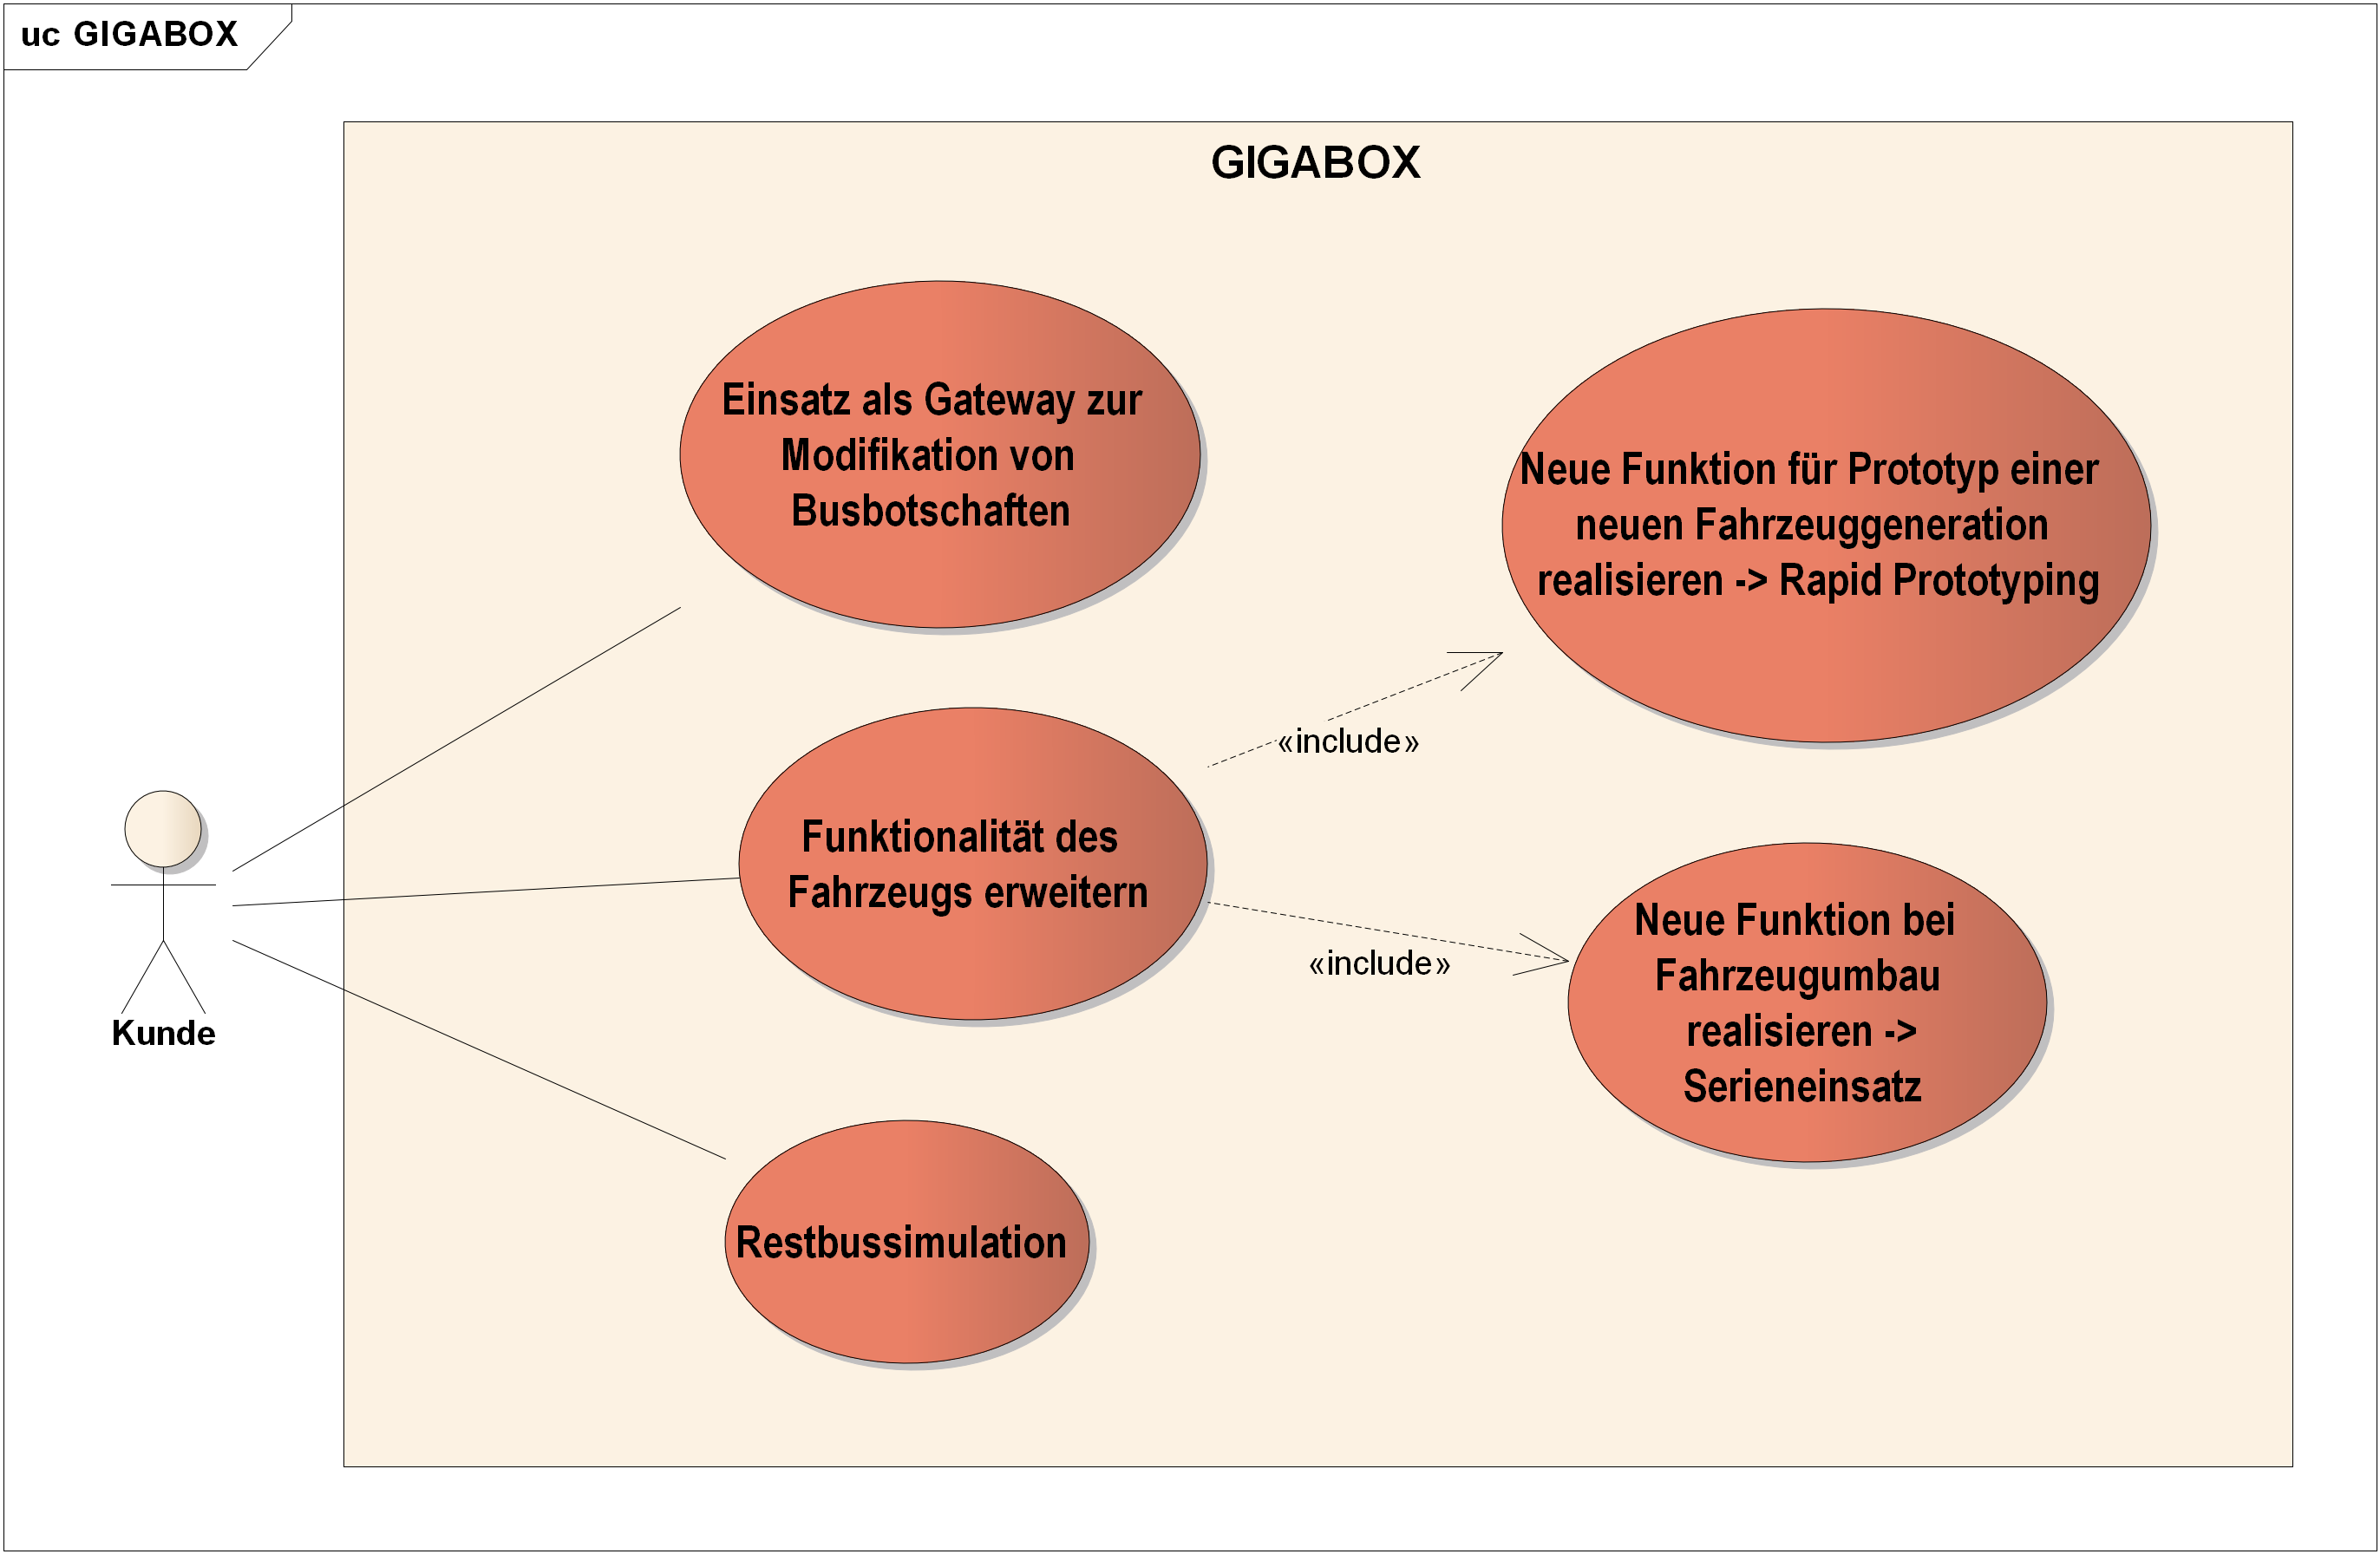
\includegraphics[width=\textwidth]{images/UseCasesGigabox.png}
	\caption{Use-Case-Diagramm GIGABOX}
	\label{fig:UseCasesGIGABOX}
\end{figure}



\subsection{Hardware der GIGABOX FD}

Die GIGABOX FD ist modular aufgebaut bestehend aus einer Basisplatine und diversen Applikationsplatinen, mit denen zus�tzliche Funktionalit�ten zur Verf�gung gestellt werden k�nnen.  
Auf der Basisplatine befindet sich ein Spannungsregler, ein 32-bit Mikrocontroller ARM Cortex M4 STM32F427IIT6, Kommunikationsschnittstellen sowie analoge und digitale Ein- und Ausg�nge.  
Der Spannungsregler wird eingesetzt, um die Batteriespannung des Fahrzeugs auf die Versorgungsspannung des Mikrocontrollers herunterzuregeln.

Der Mikrocontroller wird mit einer Taktfrequenz von 168MHz betrieben und stellt 2MB Flash Speicher sowie 192 kB SRAM + 64 kB core coupled memory (CCM) zur Verf�gung.

 

%Der Mikrocontroller besitzt folgende Features:

%\begin{itemize}
	%\item 2MB Flash Speicher und 192 kB SRAM (in Datenblatt 256+4kB including 64kB of CCM(core coupled memory))
	%\item Die Taktfrequenz betr�gt bis zu 180MHz (shruti 168Mhz)
	%\item Drei 12-Bit A/D-Wandler sowie zwei 12-Bit D/A-Wandler
	%\item 168 I/O Ports mit Interruptf�higkeit
	%\item Kommunikationsschnittstellen:
	%
	%\begin{itemize}
		%\item 3 IQuadratC Schnittstellen
		%\item 4 USART sowie 4 UART
		%\item 6 SPI
		%\item 1 SAI
		%\item 2 CAN
		%\item 1 SDIO
	%\end{itemize}
%\end{itemize}


 
Auf der GIGABOX FD sind als Kommunikationsschnittstellen 2 CAN-, 2 CAN FD- und 2 LIN-Kan�le implementiert. Zus�tzlich wird eine USB-Schnittstelle bereitgestellt, die mit einem UART-to-USB-Converter realisiert wird.
Es sind 4 analoge Eing�nge vorhanden um Sensorwerte einzulesen wie z. B. von einem Temperatursensor. Mit den 8 digitalen Eing�ngen k�nnen z. B. Schalterzust�nde eingelesen werden. Als Ausg�nge stehen 8 Halbbr�ckenausg�nge und 2 Highsideausg�nge zur Verf�gung (Wann werden Halbbr�cken- wann Highside benutzt?).  

Einen �berblick �ber die eingesetzte Hardware bietet Abbildung \ref{fig:HardwareGIGABOXFD} (Von Shruti, Abb neu erstellen wegen schlechter Bildqualit�t).

Der Einsatz von einer Applikationsplatine erm�glicht die Funktionserweiterung der GIGABOX FD um beispielsweise zus�tzliche Kommunikationsschnittstellen wie Bluetooth bereitzustellen.

\begin{figure}[!htbp]
	\centering
		\includegraphics[width=\textwidth]{images/HardwareOverviewGIGABOXFD.png}
	\caption{Hardware�berblick GIGABOX FD}
	\label{fig:HardwareGIGABOXFD}
\end{figure}


\subsection{Softwarearchitektur der GIGABOX FD}

Abbildung \ref{fig:Softwarearchitektur} gibt einen �berblick �ber die Softwarearchitektur der GIGABOX FD. 

Der Hardware Abstraction Layer (HAL) ist eine Softwareschicht, die �bergeordnete Schichten von der Hardware abstrahiert. �bergeordnete Schichten sind damit unabh�ngig von der eingesetzten Hardware. Dies bietet den Vorteil, dass bei Hardware�nderungen nur der HAL angepasst werden muss, nicht aber die �bergeordneten Schichten. Auf dem HAL sind die Treiber des Mikrocontrollers und der zugeh�rigen Peripherie implementiert. Die Treiber stellen ein Application Programming Interface (API) bereit, die Zugriff auf den Speicher oder die Peripherie des Mikrocontrollers wie z.B. Analog-Digital-Converter (ADC) erm�glicht.

Vom Middleware Layer aus kann �ber die API des Hardware Abstraction Layers auf die Hardware zugegriffen werden. Auf dieser Schicht ist ein USB-HID Treiber implementiert, der ben�tigt wird, damit die GIGABOX FD bei Verbindung mit einem Computer �ber USB als Human Interface Device (HID) erkannt wird. 
Au�erdem befindet sich dort das Transportprotokoll ISO-TP f�r CAN-Bus. Das Protokoll wird ben�tigt, um Botschaften zu verschicken, die die maximale Nutzdatengr��e von 8 Byte eines CAN-Frames �berschreiten.
Um die Pawn virtuelle Maschine (VM) an den HAL anzubinden, befindet sich auf dem Middleware Layer zus�tzlich die PAWN Driver Abstraction.

Auf dem Application Layer ist die Pawn VM und der Bootloader implementiert. Eine Abstraktionsebene �ber der Pawn VM liegt die Skript Applikation, die vom Endanwender auf den Flash-Speicher der GIGABOX FD aufgespielt werden kann. Das Skript erm�glicht die Ansteuerung bzw. Abfrage der Kommunikationsschnittstellen sowie das Steuern bzw. Beobachten der digitalen/analogen Ein-/Ausg�nge der GIGABOX FD. Auf dieser Ebene ist au�erdem die Konsole angesiedelt, an die der Anwender Befehle senden kann �ber USB.




\begin{figure}[!htbp]
	\centering
		\includegraphics[width=\textwidth]{images/GIGABOXFD_SWArchitektur.png}
	\caption{Softwarearchitektur der GIGABOX FD}
	\label{fig:Softwarearchitektur}
\end{figure}


\section{Pawn}

Pawn ist eine Skriptsprache mit einer C �hnlichen Syntax sowie eine zugeh�rige virtuelle Maschine, auf der kompilierter Pawn-Quellcode ausgef�hrt werden kann. Das Pawn-Paket, das Kompiler und virtuelle Maschine beinhaltet, ist kostenlos verf�gbar und wurde unter der Apache Lizenz 2.0 ver�ffentlicht. Die Sprache wurde abgeleitet von der Sprache "`Small-C"', die wiederum eine Teilmenge von C darstellt und f�r Mikrocontroller entwickelt wurde.
Pawn wurde erstmal 1998 �ffentlich zug�nglich gemacht, damals noch unter dem Namen "`SMALL"' und wird seitdem regelm��ig weiterentwickelt.

Pawn-Quellcode kann mithilfe des Pawn-Kompilers in Bytecode kompiliert werden. Der Bytecode wird anschlie�end auf der zugeh�rigen virtuellen Maschine interpretiert. Dies bedeutet, dass f�r jede Bytecode-Anweisung definierte Funktionen aus einer C-Klassenbibliothek aufgerufen werden. Die Ausf�hrung von Bytecode auf einer virtuellen Maschine bietet im Vergleich zur Ausf�hrung von nativem Code auf der Zielhardware den Vorteil, dass der Code unabh�ngig von der eingesetzten Hardware lauff�hig ist. Der Code kann folglich plattformunabh�ngig eingesetzt werden. Die virtuelle Maschine muss dagegen an die eingesetzte Plattform angepasst werden.
Dieser Vorteil wird allerdings mit Geschwindigkeitseinbu�en bei der Programmausf�hrung bezahlt.
Bei der Entwicklung von Pawn wurde besonders auf eine einfache Syntax, Schnelligkeit in der Codeausf�hrung und Robustheit wert gelegt. 
Die virtuelle Maschine eignet sich aus diesem Grund auch zur Einbindung in Mikrocontroller mit geringer Rechenleistung und Speicherkapazit�t.

In Bezug auf GIGABOX-Steuerger�te wird Pawn benutzt, um GIGABOX-Applikationen zu erstellen. Mithilfe von GIGABOX-Applikationen kann der Anwender Funktionen f�r GIGABOX-Steuerger�te entwickeln und die Applikation anschlie�end auf GIGABOX-Steuerger�te flashen, auf denen eine Pawn-VM implementiert ist. 
GIGABOX-Applikationen werden mithilfe eventgetriebener Programmierung entwickelt. Sobald ein definiertes Event wie z. B. der Empfang einer CAN-Botschaft eintritt, wird die dem Event zugeordnete Funktion aufgerufen.
 

\cite{PawnImplementersGuide}, \cite{PawnLanguageGuide}

Siehe Pawn\_Language\_Guide.pdf, Foreword \\
Pawn\_Implementation\_Guide.pdf, The Compiler, The abstract machine


%
%\subsection{configurAIDER}
%
%Der configurAIDER ist eine von GIGATRONIK entwickelte integrierte Entwicklungsumgebung (IDE), die es Benutzern erm�glicht, mit einer GIGABOX zu kommunizieren und diese zu programmieren. Es k�nnen Diagnoseinformationen abgerufen werden und Bytecode auf das Steuerger�t geflasht werden. Die IDE besteht aus Editoren (skriptEDITOR und multiEDITOR), Interpreter und Linker. Der scriptEDITOR ist ein Texteditor, mit dem PAWN-Skripte geschrieben werden k�nnen. Mit dem multiEDITOR k�nnen tabellarisch WENN DANN Anweisungen konfiguriert werden, aus denen ein Skript mit PAWN-Code generiert werden kann. Der multiEDITOR stellt f�r Benutzer ohne Programmierkenntnisse eine M�glichkeit dar, die GIGABOX mit rudiment�ren Funktionen zu konfigurieren. 
%Der integrierte Interpreter kann Bytecode aus den erstellten PAWN-Skripten erstellen und auf die GIGABOXEN flashen.

\section{Softwareentwicklungsprozess}
\subsection{V-Modell 97}

Das V-Modell 97 ist ein Vorgehensmodell f�r IT-Entwicklungsprojekte, das 1997 von der Bundesrepublik Deutschland ver�ffentlicht wurde. Es hat sich als Entwicklungsstandard in der Softwareentwicklung etabliert. 

Der Entwicklungsprozess nach dem V-Modell durchl�uft verschiedene Phasen. Es beginnt mit einer Anforderungsanalyse (Phase Requirements), bei der die Anforderungen an ein System ermittelt und dokumentiert werden. Anschlie�end wird das System entworfen



\begin{figure}[!htbp]
	\centering
		\includegraphics[width=0.8\textwidth]{images/V-Modell-Steps.png}
	\caption{Vorgehensschritt im V-Modell}
	\label{fig:V-Modell}
\end{figure}

\subsection{Qualit�tskriterien an Software} \label{sec:Qualit�tskriterienSW}

Um Softwarequalit�t definierbar zu machen, wurden diverse Software-Qualit�tsmodelle entwickelt. Die ISO/IEC 25010 definiert unter anderem das Product Quality Model. 
Dieses Modell definiert acht Qualit�tmerkmale f�r Software, die im folgenden erl�utert werden:

\begin{itemize}
	\item \emph{Functional Suitability:} 
	
	"`Das Qualit�tsmerkmal der funktionallen Eignung fordert, dass ein Software-System die von ihm erwartete Funktionalit�t in angemesserner und konkreter Art und Weise und unter Ber�cksichtigung der festgelegten Randbedingungen und Eigenschaften umsetzt. Dabei geht es um Fragestellungen nach der Angemessenheit der Funktionalit�ten f�r den vorgegebenen Einsatzbereich des Systems."' \cite{SWRequirements}
	
	\item \emph{Performance Efficiency}
	
	"`Das Merkmal der Performanz und Effizienz betrachtet das Leistungsniveau einer Anwendung in Abh�ngigkeit der eingesetzten Betriebsmittel und der geforderten Bedingungen. Dabei geht es insbesondere um das Zeitverhalten der Anwendung (Anwendungszeit, Durchsatz) sowie das Verbrauchsverhalten in Bezug auf Speicher, Prozessorzeit und andere Ressourcen."' \cite{SWRequirements}
	
	\item \emph{Compatibility}
	
	"`Das Merkmal der Kompatibilit�t betrachtet einerseits die explizite Zusammenarbeit des Systems mit anderen Systemen und andererseits die impliziten Auswirkungen des Systems auf andere Systeme, die auf der gleichen Hardware laufen."' \cite{SWRequirements}
	
	\item \emph{Usability}
	
	"`Das Qualit�tsmerkmal der Benutzerfreundlichkeit besch�ftigt sich damit, wie gut ein System seine Nutzer dabei unterst�tzt ihre Ziele effizient und effektiv zu erreichen. Zu den zentralen Teilmerkmalen z�hlt hier beispielsweise der Aufwand f�r die Erlernung des Systems sowie f�r die Bedienung. Ein weiteres Teilmerkmal ist die Attraktivit�t des Systems f�r die Nutzer."' \cite{SWRequirements}
	
	\item \emph{Reliability}
	
	"`Das Qualit�tsmerkmal der Zuverl�ssigkeit beschreibt die F�higkeit des Systems sein Leistungsniveau unter festgelegten Bedingungen �ber einen festgelegten Zeitraum zu bewahren. Zu den Teilmerkmalen z�hlen hier beispielsweise die Robustheit gegen�ber fehlerhaften Eingaben, die Stabilit�t beim Umgang mit fehlerhaften Systemzust�nden und die Wiederherstellbarkeit bei Systemausf�llen."' \cite{SWRequirements}
	
	
	\item \emph{Security}
	
	"`Das Merkmal umfasst alle in Bezug auf Datensicherheit relevanten Teilmerkmale wie die Datenintegrit�t, Authentizit�t und Vertraulichkeit."' \cite{SWRequirements}
	
	\item \emph{Maintainability}
	
	"`Das Merkmal der Wartbarkeit, teilweise auch als �nderbarkeit bezeichnet, besch�ftigt sich vorrangig mit der internen Qualit�t eines Systems. Zentrale Teilmerkmale hier sind der Aufwand zur Analyse eines Fehlers oder Fehlverhaltens, der Aufwand zur Durchf�hrung von Modifikationen mit entsprechender Testbarkeit sowie die Stabilit�t des Systems gegen�ber unerwarteten Seiteneffekten."' \cite{SWRequirements}
	
	\item \emph{Portability}
	
	"`Die Portabilit�t als weiteres Qualit�tsmerkmal besch�ftigt sich mit dem Aufwand, um ein System strukturell zu ver�ndern, auf eine andere Umgebung zu verlagern oder einzelne Systemkomponenten auszutauschen. Als Teilmerkmale nennt der Standard die Anpassbarkeit eines Systems an unterschiedliche Umgebungen, den Aufwand zur Installation und die Austauschbarkeit von Komponenten."' \cite{SWRequirements}
	
\end{itemize}
 



Abbildung \ref{fig:ProductQualityModel} zeigt eine �bersicht �ber die acht Qualit�tsmerkmale und l�st jedes Merkmal feingranular weiter auf.


\begin{figure}[!htbp]
	\centering
		\includegraphics[width=\textwidth]{images/ProductQualityModel.png}
	\caption{Qualit�tsmerkmale des Product Quality Model nach ISO/IEC 25010}
	\label{fig:ProductQualityModel}
\end{figure}


Um das Qualit�tsmerkmal "`Usability"' zu verfeinern, kann die Norm EN ISO 9241-110 (Grunds�tze der Dialoggestaltung) herangezogen werden.
Diese beschreibt, welche Eigenschaften Dialoge erf�llen sollen, um eine gute Usability zu erreichen. Die sieben Grunds�tze der Dialoggestaltung werden im Folgenden nach Quelle \cite{MCInteraktion}, Kapitel 8.3 zitiert.



	
\begin{itemize}
		\item Aufgabenangemessenheit: "`Ein interaktives System ist \textit{aufgabenangemessen}, wenn es den Benutzer unterst�tzt, seine Arbeitsaufgabe zu erledigen, d.h. wenn Funktionalit�t und Dialog auf den charakteristischen Eigenschaften der Arbeitsaufgabe basieren, anstatt auf der zur Aufgabenerledigung eingesetzten Technologie."'
		
		\item Selbstbeschreibungsf�higkeit: "`Ein Dialog ist in dem Ma�e \textit{selbstbeschreibungsf�hig}, in dem f�r den Benutzer zu jeder Zeit offensichtlich ist, in welchem Dialog, an welcher Stelle er sich befindet, welche Handlungen unternommen werden k�nnen und wie diese ausgef�hrt werden k�nnen."'
		
		\item Lernf�rderlichkeit: "`Ein Dialog ist \textit{lernf�rderlich}, wenn er den Benutzer beim Erlernen der Nutzung des interaktiven Systems unterst�tzt und anleitet."'
		
		\item Steuerbarkeit: "`Ein Dialog ist \textit{steuerbar}, wenn der Benutzer in der Lage ist, den Dialogablauf zu starten sowie seine Richtung und Geschwindigkeit zu beeinflussen, bis das Ziel erreicht ist."'
		
		\item Erwartungskonformit�t: "`Ein Dialog ist \textit{erwartungskonform}, wenn er den aus dem Nutzungskontext heraus vorhersehbaren Benutzerbelangen sowie allgemein anerkannten Konventionen entspricht."'
		
		\item Individualisierbarkeit: "`Ein Dialog ist \textit{individualisierbar}, ween Benutzer die Mensch-System-Interaktion und die Darstellung von Informationen �ndern k�nnen, um diese an ihre individuellen F�higkeiten und Bed�rfnisse anzupassen.
		
		\item Fehlertolerant:  "`Ein Dialog ist \textit{fehlertolerant}, wenn das beabsichtigte Arbeitsergebnis trotz erkennbar fehlerhafter Eingaben entweder mit keinem oder mit minimalem Korrekturaufwand durch den Benutzer erreicht werden kann."'


	Quelle: Wikipedia -> �berpr�fen ob andere Quelle verf�gbar ist, am Besten die Norm direkt
	Als Quelle kann Paper von PH Weingarten "`Usability und Usability Engineering genommen werden"'. Hieraus die Stichpunkte noch verfeinern

\end{itemize}

\section{Entwicklungsframework}

\subsection{.NET Framework}

Es wurden im folgenden Abschnitt die Quellen \cite{Louis:CSharp},\cite{msdn} verwendet.

Das .NET Framework ist eine von Microsoft entwickelte Entwicklungsplattform f�r Anwendersoftware, die erstmals im Januar 2002 in der Version 1.0 erh�ltlich war. Es stellt die Umsetzung des Common Language Infrastructure (CLI) Standards dar, der sprach- und plattformunabh�ngige Anwendungsentwicklung spezifiziert.
Wesentliche Bestandteile des .NET Frameworks sind die Laufzeitumgebung Common Language Runtime (CLR) und die Framework Class Library (FCL). 
Die CLR verwaltet Speicher, Thread- und Codeausf�hrung, �berpr�fung der Codesicherheit und Kompilierung. Von der CLR verwalteter Code wird dabei Managed Code genannt, au�erhalb der CLR laufender Code Unmanaged Code. Es wird eine Vielzahl von Programmiersprachen unterst�tzt, unter anderem C\#, C++ und Visual Basic .NET. Beim Kompilieren der verschiedenen Hochsprachen wird der Code zun�chst in eine Zwischensprache �bersetzt, der Common Intermediate Language (CIL). Aus dem daraus entstehenden Intermediate Language Code (IL-Code) wird dann von einem Just-In-Time-Compiler (JIT-Compiler) zur Laufzeit Maschinencode erzeugt (Abbildung \ref{fig:NET-Framework}).

\begin{figure}[!htbp]
	\centering
		\includegraphics[width=0.8\textwidth]{images/NET-Framework.jpg}
	\caption{Managed Code und Unmanaged Code}
	\label{fig:NET-Framework}
\end{figure}

Die FCL ist eine objektorientierte Klassenbibliothek mit einer Auflistung wiederverwendbarer Typen, von denen eigener Code abgeleitet werden kann.  


\subsection{Windows Presentation Framework (WPF)}

Mit Einf�hrung des .NET Frameworks 3.0 im Jahr 2006 wurde Windows Presentation Foundation (WPF) ver�ffentlicht, ein Framework zur Erstellung von grafischen Benutzeroberfl�chen. WPF stellt den Nachfolger f�r das seit Version 1.0 im .NET Framework enthaltene Windows Forms. Es k�nnen Desktop- sowie Webanwendungen erstellt werden. 

WPF nutzt die Leistungsressourcen von Grafikkarten mit 3D-Beschleunigern besser aus als Windows Forms, da zum Rendern der GUI-Inhalte DirectX benutzt wird anstatt Graphics Device Interface+ (GDI+). Mithilfe von DirectX kann WPF grafische Elemente selbst zeichnen anstatt dass sie durch das Betriebssystem gezeichnet werden.  
Ein weiterer Vorteil von WPF ist das vektorbasierte Zeichnen der Anwendungsinhalte. Dies erm�glicht eine beliebige Skalierung der Inhalte ohne Verpixelung.

Eines der zentralen Konzepte von WPF ist die Verwendung der XML-basierten Beschreibungssprache Extensible Application Markup Language (XAML) zur Beschreibung der Benutzeroberfl�che. XAML erm�glicht eine �bersichtlichere und kompaktere Beschreibung der Benutzeroberfl�che als die Programmierung der Oberfl�che in C\#. 

Die Beschreibung einer Benutzeroberfl�che mit XAML wird in einer XAML-Datei vorgenommen. 
Jede XAML-Datei ist untrennbar mit einer Codebehind-Datei gekoppelt, in der die Logik der Benutzeroberfl�che in C\# programmiert werden kann.
Die Logik kann allerdings auch in einer eigenen C\#-Quellcodedatei programmiert werden und �ber sogenannte DataBindings und Commands an die XAML-Datei angebunden werden.
Darstellung und Logik k�nnen auf diese Weisen getrennt werden, was unter anderem eine effektivere Zusammenarbeit zwischen Designern der Benutzeroberfl�che und Entwicklern der Anwendungslogik erm�glicht. 

Ein Designer kann mithilfe eines Design-Tools wie z. B. Microsoft Expression Blend die Benutzeroberfl�che entwerfen und daraus eine XAML-Datei generieren. 
Der Entwickler der Anwendungslogik kann anschlie�end auf Grundlage der XAML-Datei des Designers die gew�nschte Logik zu der GUI entwickeln.

 


 	
	\chapter{Anforderungsanalyse} \label{chp:Anforderungsanalyse}

\section{�berblick}

In diesem Kapitel soll eine Anforderungsanalyse f�r eine Entwicklungsumgebung f�r GIGABOX-Steuerger�te durchgef�hrt werden.
In Abbildung \ref{fig:UseCasesGIGABOX} wurde gezeigt, f�r welche Anwendungen GIGABOXEN eingesetzt werden. 
Die Anforderungen an die Entwicklungsumgebung wurden so gestellt, dass sie Softwareentwicklern f�r GIGABOX-Funktionen die Umsetzung dieser Anwendungen erm�glicht und m�glichst gro�e Unterst�tzung bei der Codeentwicklung bietet.

Zuerst wurden Gespr�che Gespr�che mit Entwicklern gef�hrt, vorhandener Programmcode aus realisierten Projekten analysiert und selbstst�ndig Codeentwicklung mit dem bestehenden configurAIDER betrieben um herauszufinden, welche Use Cases eine IDE zur Entwicklung von Funktionen f�r GIGABOX-Steuerger�te abdecken soll. Aus dieser Analyse entstanden die in Abbildung \ref{fig:UseCases} veranschaulichten Use-Cases.

\begin{figure}[!htbp]
	\centering
		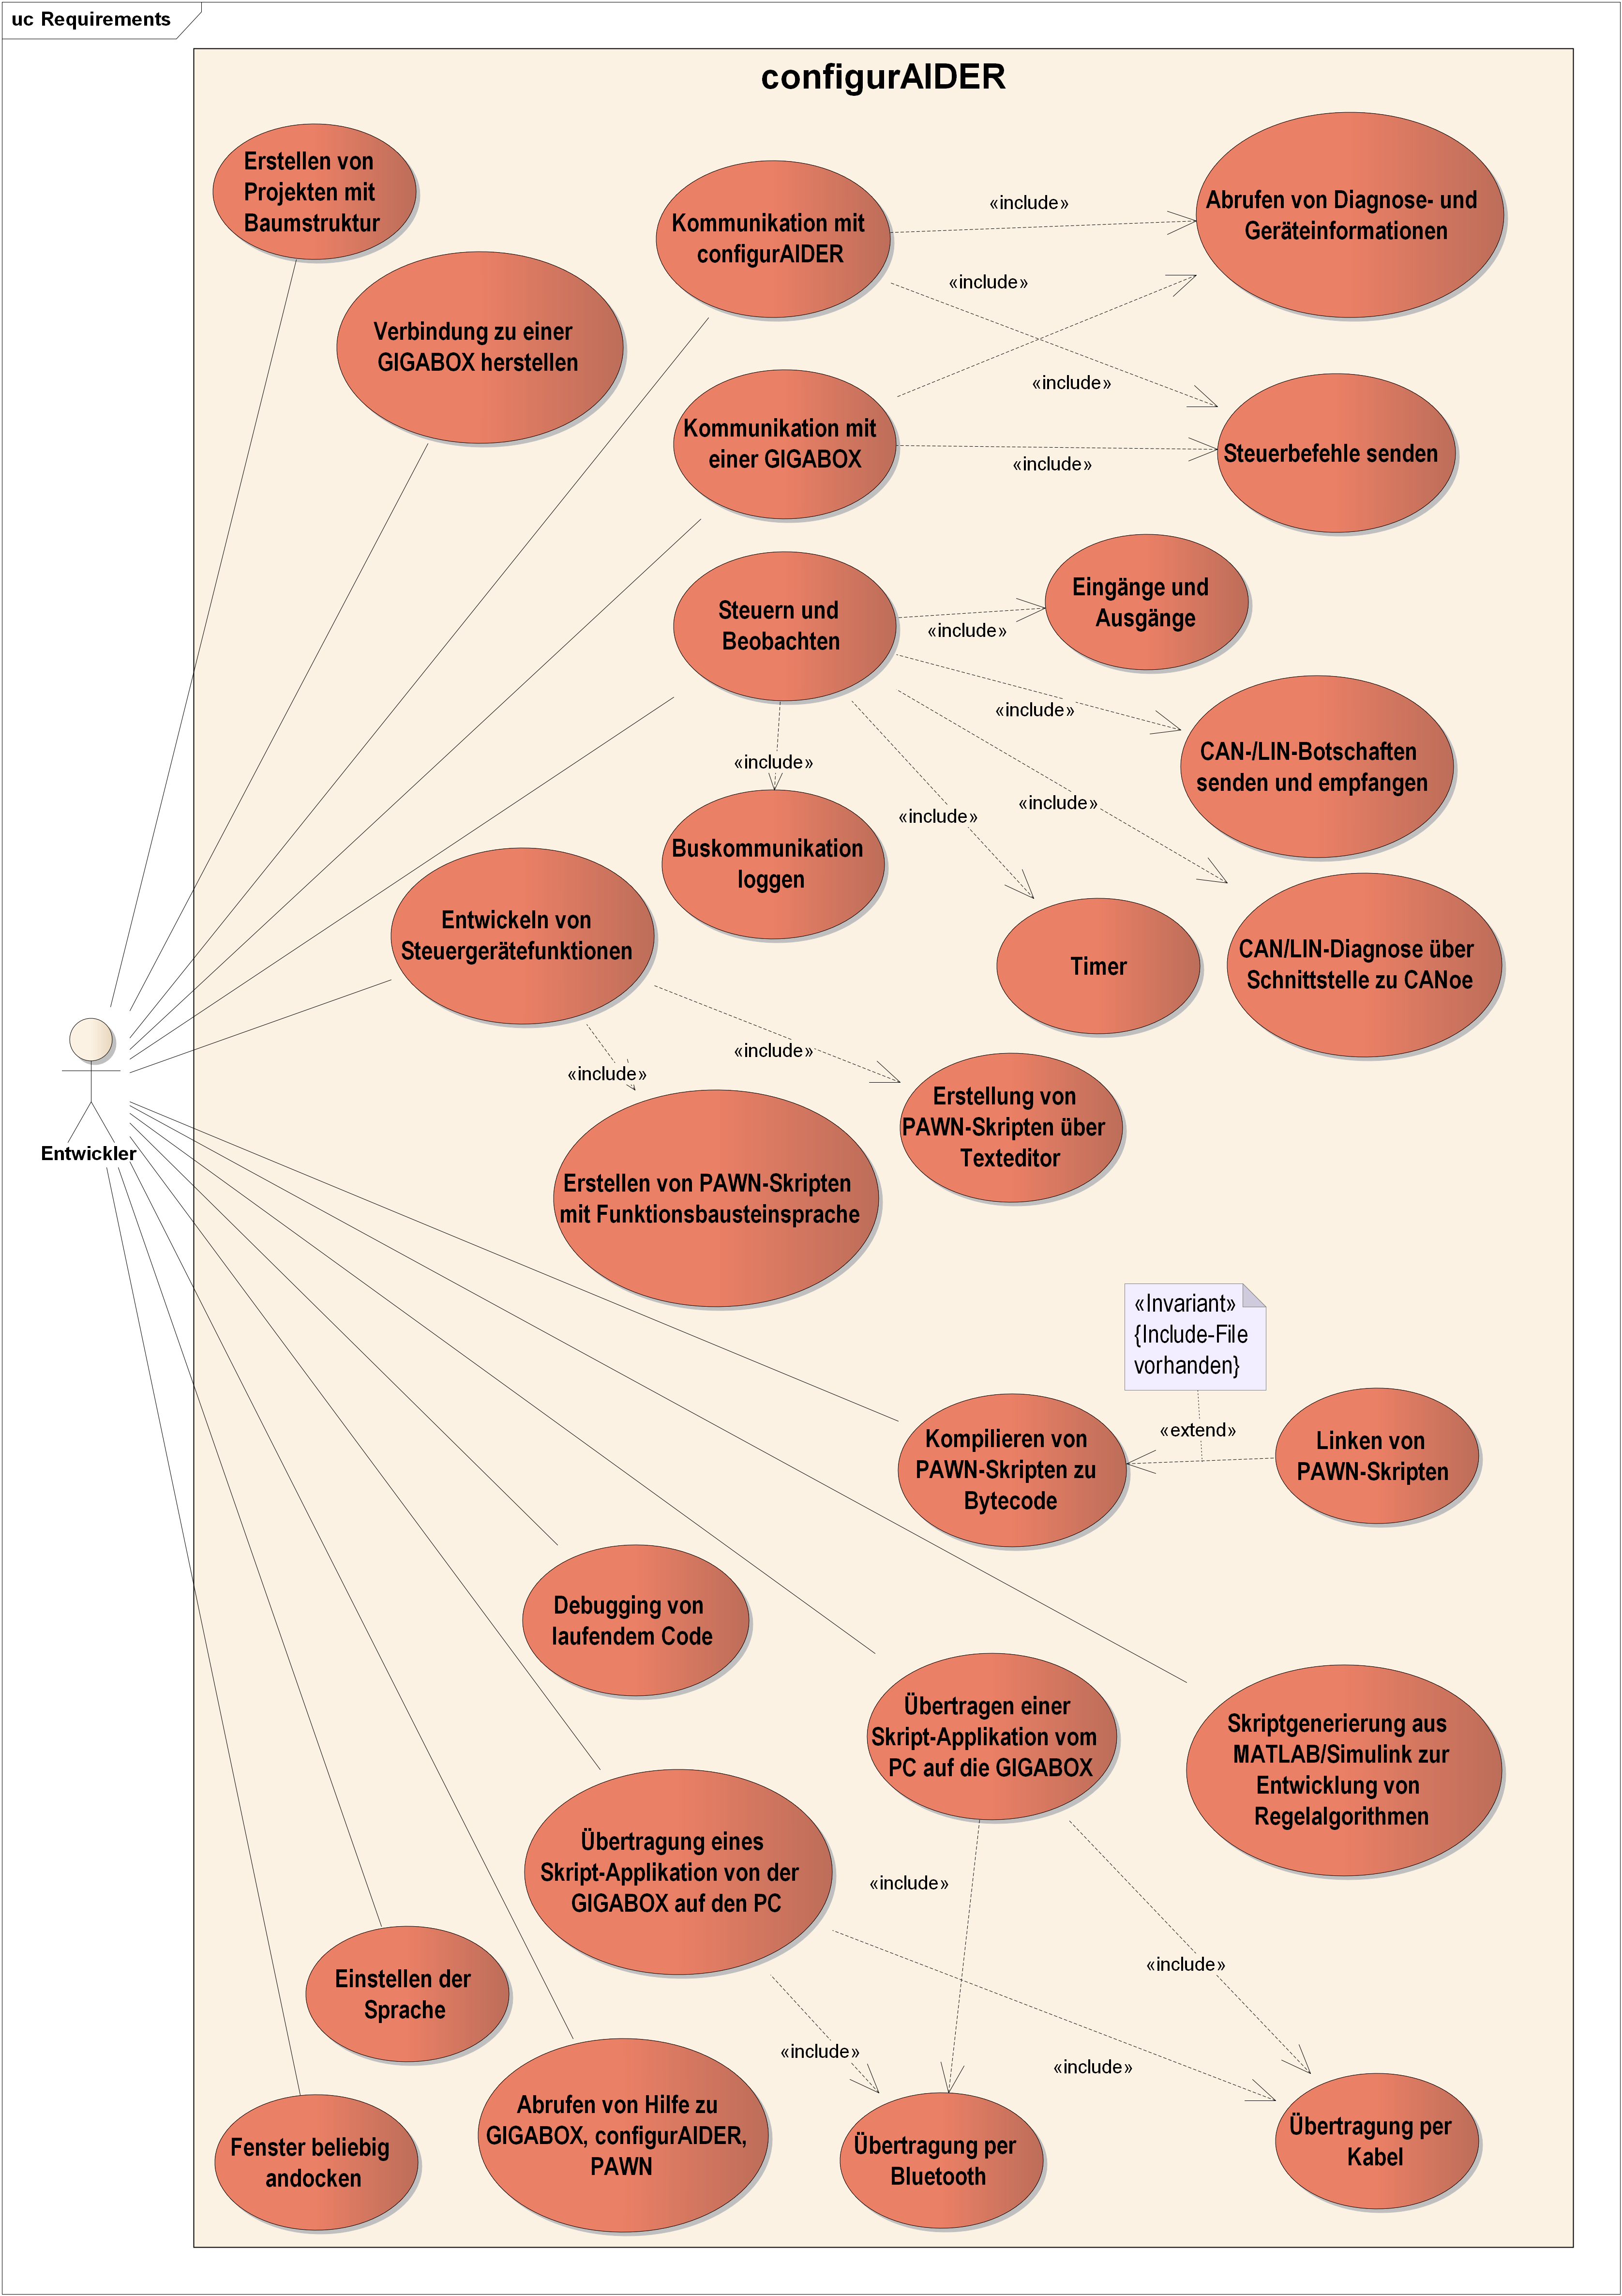
\includegraphics[width=\textwidth]{images/RequirementsUseCases.png}
	\caption{Use-Case-Diagramm funktionale Anforderungen}
	\label{fig:UseCases}
\end{figure}


Von den ermittelten Use Cases wurden direkt die funktionalen Anforderungen abgeleitet, die im folgenden Abschnitt n�her beleuchtet werden.

Auf Basis der Qualit�tsmerkmale f�r die Anforderungsspezifikation im Standard IEEE 830-1998 werden die ermittelten funktionalen Anforderungen eingeteilt in drei Priorit�rsklassen: 

\begin{itemize}
	\item Essential: Das Software-System kann nicht akzeptiert werden, wenn diese Anforderung nicht in der vereinbarten Form geliefert wird.
	\item Conditional: Diese Anforderungen erweitern das Software-System in geeigneter Form. Wenn sie fehlen, w�rden sie den Einsatz des Systems jedoch nicht gef�hrden.
	\item Optional: Diese Anforderungen sind nicht unbedingt notwendig, f�r die Anwender jedoch eine angenehme Erweiterung (nice to have).

\end{itemize}





Zur Ermittlung der nichtfunktionalen Anforderungen wurden bekannte Vorgehensmodelle und Normen der Softwareentwicklung herangezogen.  
Die hergeleiteten nichtfunktionalen Anforderungen sollen bei der Entwicklung beachtet werden, um eine hohe Qualit�t der zu entwickelnden Software sicherzustellen. Auf eine Bewertung wird verzichtet.

Quelle: \cite{SWRequirements}

\section{Ermittlung und Bewertung von funktionalen Anforderungen}

\subsection{Erstellung von Projekten mit Baumstruktur} \label{sec:ProjekteErstellen}

\emph{Beschreibung}: 

Innerhalb eines Projektes k�nnen verschiedene GIGABOX-Modelle angelegt werden. F�r jedes angelegte GIGABOX-Modell k�nnen PAWN-Skripte erstellt werden mit der zum Modell passenden Dateiendung .p. F�r jedes angelegte GIGABOX-Modell k�nnen Include-Files hinzugef�gt werden.
Der Benutzer erh�lt einen strukturierten �berblick �ber alle seine GIGABOX-Projekte und alle f�r ein Projekt entwickelten Skripte. Das �ffnen eines Skriptes erfolgt komfortabel �ber Doppelklick auf ein Skript in der Projektstruktur. L�stiges navigieren durch die Dateistruktur des PCs beim �ffnen eines Skriptes entf�llt + der Benutzer muss den Ablageort im Dateisystem nicht wissen. 

\emph{Bewertung}:

Erh�ht den Benutzerkomfort signikfikant, deshalb Einstufung in Priorit�tsklasse "`Conditional"'.


\subsection{Einstellung der Sprache}

\emph{Beschreibung}:

Die Sprache der Benutzeroberfl�che kann angepasst werden. Es soll Deutsch und Englisch zur Verf�gung stehen. 

\emph{Bewertung}:

Die Darstellung der Benutzeroberfl�che in der Muttersprache des Benutzers erh�ht die Usability, da es die Selbstbeschreibungsf�higkeit und Individualisierbarkeit f�rdert. Englisch muss auf jeden Fall zur Verf�gung stehen, da es die international am weitesten verbreitete Sprache ist und auch in Deutschland von einem Gro�teil der Menschen verstanden wird. Die Darstellung der Benutzeroberfl�che in Englisch wird deshalb in Priorit�tsklasse "`Essential"' eingeteilt. 
Die Darstellung in Deutsch wird in Klasse "`Optional"' eingeteilt, da die Usability dadurch nur m��ig erh�ht wird. 
Das liegt daran, dass der potenzielle Benutzerkreis des Tools Entwickler sind, denen gr��tenteils der Umgang mit englischen GUIs vertraut ist.

\subsection{Texteditor zur Erstellung von PAWN-Skripten}

\begin{itemize}
	\item Schreiben von PAWN-Code
	
	\emph{Beschreibung:}
	
	Es steht ein Textfeld zur Verf�gung, in dem PAWN-Code editiert werden kann.
	
	\emph{Bewertung:}
	
	Klasse "`Essential"', da als Grundfunktionalit�t einer IDE einzustufen.
	
	\item Copy/Paste
	
	\emph{Beschreibung:}
	
	Codefragmente k�nnen kopiert und an anderer Stelle eingef�gt werden. 
	
	\emph{Bewertung:}
	
	Macht die Codeentwicklung bedeutend effektiver, da dem Benutzer Tipparbeit erspart bleibt. Weiterer Vorteil ist die Fehlervermeidung durch Tippfehler. Deshalb Einstufung in Klasse "`Conditional"'. 

	\item Suchen/Ersetzen
	
	\emph{Beschreibung:} 
	
	Ein Skript kann nach Zeichenketten durchsucht werden. Die gefundenen Ergebnisse werden farblich hervorgehoben und es kann zu den Ergebnissen gesprungen werden. Alle gefundenen Ergebnisse k�nnen ersetzt werden durch eine neue Zeichenkette. 
	
	\emph{Bewertung:}
	
	Das Auffinden von Variablen und Methoden im Skript wird erheblich erleichtert. Bei Umbenennung von Variablen oder Methoden wird viel Zeit eingespart und es werden Tippfehler vermieden. Einteilung in Klasse "`Conditional"'.
	
	\item Letzte Schritte r�ckg�ngig machen
	
	\emph{Beschreibung:}
	
	Die letzten vom Benutzer vorgenommenen Anweisungen k�nnen r�ckg�ngig gemacht werden.
	
	\emph{Bewertung:}
	
	F�rdert die Fehlertoleranz. Einteilung in Klasse "`Conditional"'
	
	\item Paralleles �ffnen von Skripten	
	
	\emph{Beschreibung:}
	
	Mehrere Skripte lassen sich parallel �ber Tabs �ffnen.
	
	\emph{Bewertung:}
	
	Erh�ht die Usability (effektives arbeiten). Es kann einfacher Code zwischen verschiedenen Skripten kopiert werden. Klasse "`Conditional"'
	
	
	\item Anzeige aller instanziierten Variablen im Skript
	
	\emph{Beschreibung:}
	
	Alle instanziierten Variablen werden aufgelistet. Doppelklick auf einen Variablennamen in der Liste markiert im Skript alle Verwendungen der Variable. Per Drag\&Drop kann ein Variablenname aus der Liste in das Skript eingef�gt werden.
				
	\emph{Bewertung: }

	Benutzer hat alle instanziierten Variablen im Blick und kann leicht zu Verwendungsstellen im Skript navigieren. Das Einf�gen per Drag\&Drop bietet eine komfortable M�glichkeit der Variablenverwendung und verhindert Fehleingaben durch Tippfehler. 
	Einteilung in Klasse "`Optional"'.
	
	\item Anzeige aller implementierten Funktionen zur Navigation im Skript
	
	\emph{Beschreibung:}
	
	Alle implementierten Funktionen werden gelistet. Doppelklick auf eine Funktion f�hrt zu einem Sprung zur Funktionsimplementierung. Per Drag\&Drop kann ein Funktionsname in das Skript gezogen werden, ein Aufruf der Funktion wird in das Skript eingef�gt. Es k�nnen alle Stellen im Skript markiert werden, an denen die gew�hlte Funktion aufgerufen wird.
	
\emph{Bewertung:}
	
	Benutzer hat alle implementierten Funktionen im Blick und kann leicht zu Verwendungsstellen im Skript navigieren. Komfortable M�glichkeit der Funktionsverwendung, Verhindert Fehleingaben durch Tippfehler.
	Einteilung in Klasse "`Optional"'.
	
	\item Bei der Codeentwicklung unterst�tzende Funktionen
	
	\emph{Beschreibung:} 
	
	Es sollen Funktionen integriert werden, die schnelleres und effektiveres Schreiben von Code erm�glichen.
	Bsp: Autovervollst�ndigung von Variablen, Funktionen und Anweisungen bei der Tastatureingabe
	
	\emph{Bewertung: }
	
	Einteilung in Klasse "`Conditional"'.
	
	\item Routingeditor
	
	\emph{Beschreibung:}
	
	\textcolor[rgb]{1,0,0}{Beschreibung f�r CAN hier. Auch f�r LIN gibt es Dokumente, die Botschaften definieren. Die Dokumente k�nnten geparst werden und darauf ein PAWN-Skript generiert werden, das die Botschaften als Variablen enth�lt.}
	
	
	Aus einer Datenbankdatei (.dbc/.arxml) k�nnen dort definierte Bussignale geladen werden. Die Signale k�nnen in verschiedenen CAN-Botschaften enthalten sein. 	
	Aus den Bussignalen kann im Routingeditor eine eigene CAN-Busbotschaft konfiguriert werden mit einer vom Benutzer definierten ID. Dazu k�nnen die Signale innerhalb der Nutzdatenfeldes einer PDU frei angeordnet werden.   
	
	Aus der im Routing-Editor konfigurierten Botschaft kann PAWN-Code generiert werden und in die Funktion OnCanRxEvent() eines ge�ffneten Skriptes im Texteditor eingef�gt werden.
	
	\emph{Bewertung:}
	
	Beim Programmieren der GIGABOX tritt des �fteren der Use-Case auf, dass aus Signalen, die in verschiedenen auf dem Bus ankommenden Botschaften enthalten sind, eine neue Botschaft erstellt und verschickt werden soll.
	
	Dabei werden oft Bitverschiebungen ben�tigt, deren Programmierung viel Zeit- und Denkaufwand bedeuten. 
	Der Routingeditor erm�glicht die grafische Konfiguration von Busbotschaften und erleichtern die Umsetzung dieser Routingaufgaben.
	Einteilung in Klasse "`Optional"'.
	
	
	
	
\end{itemize}
 
\subsection{Konfigurieren einer GIGABOX ohne PAWN-Kenntnisse}

 \emph{Beschreibung:}

	Grundlegende Funktionen einer GIGABOX sollen ohne Kenntnisse von PAWN konfiguriert werden k�nnen. 
	Dazu bietet sich die Funktionsbausteinsprache an.

\emph{Bewertung:}

Erleichtert es Kunden ohne Programmierkenntnisse, selbst�ndig GIGABOX-Funktionalit�ten zu konfigurieren. Erweitert m�glicherweise den Kreis an potentiellen K�ufern der GIGABOX. 
Im Vergleich zur direkten Codeentwicklung k�nnen allerdings nur eingeschr�nkte Funktionalit�ten realisiert werden. Erfahrene Softwareentwickler werden aufgrund dieser Tatsache PAWN-Code direkt entwickeln. 
Einteilung in Klasse "`Optional"'.

\subsection{Verbundene GIGABOXEN auflisten} \label{sec:GIGABOXENauflisten}


		
	\emph{Beschreibung:} 
	
	Alle GIGABOXEN, die mit dem PC per USB oder Bluetooth verbunden sind, werden aufgelistet. Es werden Ger�teinformationen wie z.B. Modellname, Seriennummer bereitgestellt. Der Benutzer kann aus der Liste eine GIGABOX anw�hlen, mit der kommuniziert werden soll.	
	
	\emph{Bewertung:}	
	
	
	Verbindung zu GIGABOX per USB herstellen wird als Grundfunktionalit�t eingestuft, Klasse "`Essential"'. 
	Verbindung per Bluetooth wird in Klasse "`Optional"' eingestuft.

	




\subsection{Kompilieren von Pawn-Quellcodedateien} \label{sec:Kompilieren}

	\emph{Beschreibung:}
	
	PAWN-Skripte k�nnen in Bytecode �bersetzt werden. 
	Wenn Include-Files verwendet werden, soll ein Linker den Bytecode des Skriptes und des Include-Files nach dem �bersetzen zusammenf�gen. 
	
	\emph{Bewertung:}
	
	Das Kompilieren ist eine Grundfunktionalit�t und wird deshalb in die Klasse "`Essential"' eingestuft.




\subsection{Beschreiben/Auslesen des Flash-Speichers der GIGABOX} \label{sec:FlashenGIGABOX}

	\emph{Beschreibung:}
	
Kompilierte	Skript-Applikationen k�nnen vom PC auf den Flash-Speicher einer GIGABOX �bertragen werden. Sich bereits auf dem Flash-Speicher befindliche Skripte k�nnen auf den PC geladen und angezeigt werden. Die �bertragung soll jeweils per Kabel �ber die USB-Schnittstelle und per Bluetooth m�glich sein.
	
	
	\emph{Bewertung:}

	Die �bertragung von Skripten vom PC auf eine GIGABOX �ber die USB-Schnittstelle wird als Grundfunktionalit�t bewertet und in Klasse "`Essential"' eingeteilt. Die �bertragung von der GIGABOX auf den PC �ber die USB-Schnittstelle ist f�r den Entwickler sehr n�tzlich, aber nicht unbedingt notwendig und wird deshalb als Klasse "`Conditional"' eingestuft.
Bluetooth-�bertragung wird in Klasse "`Optional"' eingestuft, da es wenige Use-Cases gibt, bei denen eine Funk�bertragung Vorteile gegen�ber der Kabel�bertragung bietet. Ein m�glicher Use-Case w�re eine schwer zug�ngliche GIGABOX im Fahrzeug, auf die ein neues Skript aufgespielt werden soll. Eine �bertragung per Bluetooth w�rde einen aufw�ndigen Ausbau der GIGABOX aus dem Fahrzeug ersparen.	


\subsection{Kommunikation mit einer GIGABOX} \label{sec:KommunikationMitGIGABOX}

	\emph{Beschreibung:}
	
	Benutzer soll Befehle an eine GIGABOX senden k�nnen, z. B. einen Reset der GIGABOX veranlassen, den Bootloader aufrufen. Au�erdem sollen Diagnose- und Ger�teinformationen abgerufen werden k�nnen. Die Daten�bertragung soll per Kabel �ber die USB-Schnittstelle und per Bluetooth m�glich sein.
	
	
	\emph{Bewertung:}
	
	Das Senden von Befehlen und Abrufen von Diagnose- und Ger�teinformationen per Kabel �ber die USB-Schnittstelle wird in Klasse "`Essential"' eingestuft. Die Daten�bertragung per Bluetooth wird in Klasse "`Optional"' eingestuft, da es wenige Use-Cases gibt, bei denen eine Funk�bertragung Vorteile gegen�ber der Kabel�bertragung bietet. Ein m�glicher Use-Case w�re eine schwer zug�ngliche GIGABOX im Fahrzeug, auf die ein neues Skript aufgespielt werden soll. Eine �bertragung per Bluetooth w�rde einen aufw�ndigen Ausbau der GIGABOX aus dem Fahrzeug ersparen.


\subsection{Kommunikation mit dem Benutzer}

	\emph{Beschreibung:}
	
	Benutzer soll Befehle �ber die Konsole an die IDE senden k�nnen, z. B. das Kompilieren eines Skriptes veranlassen.
	Au�erdem sollen Diagnose- und Programminformationen der IDE abgerufen werden k�nnen.
	
	
	\emph{Bewertung:}

	Einstufung in Klasse "`Essential"'.


\subsection{Steuern und Beobachten von Ein-/Ausg�ngen und Timern}


	\emph{Beschreibung:}
	
	Die Zust�nde der digitalen und analogen Ausg�nge sowie der internen Timer sollen �ber die Oberfl�che der Entwicklungsumgebung gesteuert und beobachtet werden k�nnen. 
	Die Zust�nde der digitalen und analogen Eing�nge sollen �ber die Oberl�che der Entwicklungsumgebung beobachtet werden k�nnen. 
	Au�erdem sollen vom Benutzer konfigurierte CAN- und LIN-Botschaften �ber die IDE gesendet werden k�nnen. Dabei soll einmaliges und zyklisches Senden von Botschaften m�glich sein. 
	Auf dem Bus liegende Botschaften einer definierten ID (CAN) bzw. f�r eine definierte Adresse (LIN) sollen beobachtet werden k�nnen.
	
	Zus�tzlich soll die M�glichkeit bestehen, Buskommunikation innerhalb eines definierten Zeitfensters mitzuloggen. Alle Busbotschaften, die innerhalb dieses Zeitfensters auf dem Bus liegen, sollen dabei mit Zeitstempel gelistet werden. 

	\emph{Bewertung:}
	
Die beschriebenen Funktionen sind f�r den Nutzer hilfreich bei der Codeentwicklung, aber nicht unbedingt notwendig. 
Damit k�nnen die Funktionen in die Priorit�tsklasse "`Optional"' eingeteilt werden.


\subsection{Debugging}


	\emph{Beschreibung:}
	
Es sollen Breakpoints gesetzt werden k�nnen. Wenn ein Breakpoint erreicht wird, wird die Codeausf�hrung auf der virtuellen Maschine der GIGABOX angehalten. Da der Codeausf�hrung eventbasiert ist, werden die gesetzten Breakpoints nur erreicht, wenn das Event ausgel�st wird, in dem sich der Breakpoint befindet. Events, die ausl�sen w�hrend die Codeausf�hrung angehalten ist, m�ssen  ignoriert werden. -> f�hrt zu Problemen, da Timer ablaufen aber nicht neu aufgezogen werden -> Timerevents m�ssten trotzdem im Hintergrund ausl�sen und neu aufgezogen werden.
Aber Anweisungen in den Event au�er TimerSet() werden ignoriert.

 CAN und LIN-Events werden ignoriert.

Der Benutzer kann zeilenweise zu den folgenden Anweisungen springen. 

	\emph{Bewertung:}
	
	Die beschriebenen Funktionen sind f�r den Nutzer hilfreich bei der Codeentwicklung, aber nicht unbedingt notwendig. 
Damit k�nnen die Funktionen in die Priorit�tsklasse "`Optional"' eingeteilt werden.
	

\subsection{Bereitstellung von Dokumentationen} \label{sec:BereitstellungDoku}

	\emph{Beschreibung:}
	
	Die IDE soll Hilfedokumentation zu den GIGABOX-Modellen, zum configurAIDER und zu PAWN bereitstellen.
	
	
	\emph{Bewertung:}
	
	Ein direkter Zugriff von der IDE aus auf die Hilfedokumentation erh�ht die Usability.
	Dies bietet dem Benutzer den Vorteil, dass er die Oberfl�che der IDE nicht verlassen muss um Dokumentationen 
	aufzurufen.	
  Einteilung in Klasse "`Conditional"'.



\subsection{Individualisierbare Oberfl�che}

	\emph{Beschreibung:}
	
	Die Fenster innerhalb der IDE sind frei andockbar. Somit kann der Benutzer die Oberfl�che individuell nach seinen W�nschen aufbauen.
	
	\emph{Bewertung:}

	Steigert die Usability (Individualisierbarkeit), ist aber keine unbedingt notwendige Funktion und wird deshalb als "`Optional"' eingestuft.


\section{Ermittlung von nichtfunktionalen Anforderungen}

\begin{itemize}
	\item Entwicklung des Tools mit WPF unter Verwendung MVVM-Pattern
	\item Entwicklung f�r Windows 32bit + 64bit  als Zielbetriebssystem
	\item Entwicklung nach V-Modell
	\item Qualit�tskriterien an Software nach ISO 9126 (aus Wiki)/ siehe auch Kapitel 6 Moderne Softwarearchitektur



	\begin{itemize}
		\item Wartbarkeit
		\begin{itemize} 
			\item Analysierbarkeit:
			
			Coding-Richtlinien sollen eingehalten werden: Verst�ndliche Kommentare, einheitliche Namensgebung etc
			\item Modifizierbarkeit:
			
			SOLID-Prinzipien einhalten, um m�glichst wenig Abh�ngigkeiten unter den Klassen zu erreichen. Dadurch treten bei Modifikationen innerhalb einer Klasse weniger schwer vorhersehbare Fehler auf 
			
			\item Testbarkeit:
			
			\textcolor[rgb]{1,0,0}{Keine Ahnung auf was bei der Entwicklung geachtet werden soll um gute Testbarkeit zu erreichen}
		\end{itemize}
			
		\item Benutzbarkeit (genauer definiert in Norm EN ISO 9241-110)
		
		\item Effizienz
			
			\begin{itemize}
				\item Akzeptable Zeit bis Tool gestartet ist und verwendbar ist
				\item Unmittelbare und fl�ssige Reaktion auf Benutzereingaben
			\end{itemize}
		
		\item �bertragbarkeit
			
			\begin{itemize}
				\item Anpassbarkeit: M�glichkeit, Software an verschiedene Umgebungen anzupassen
				
				Verschiedene Betriebssysteme? 32/64Bit?
			\end{itemize}
		
		\item Zuverl�ssigkeit
		
		\begin{itemize}
			\item Reife: Geringe Versagensh�ufigkeit durch Fehlerzust�nde:
				Ausreichendes Testing
			\item Wiederherstellbarkeit: F�higkeit, bei einem Versagen das Leistungsniveau wiederherzustellen und die direkt betroffenen Daten wiederzugewinnen. Zu ber�cksichtigen sind die daf�r ben�tigte Zeit und der ben�tigte Aufwand.
		\end{itemize}

		
	\end{itemize}

\end{itemize}






























	\chapter{Ist-Zustand}

\section{�berblick}

In diesem Kapitel wird der Ist-Zustand des configurAIDERs beschrieben. Es wird die Benutzeroberfl�che vorgestellt und die Funktionalit�t beschrieben. Im Anschluss wird die Funktionalit�t und die Usability bewertet. Abbildung \ref{fig:Uebersicht} veranschaulicht die Module, die im configureAIDER enthalten sind.

\begin{figure}[!htbp]
	\centering
		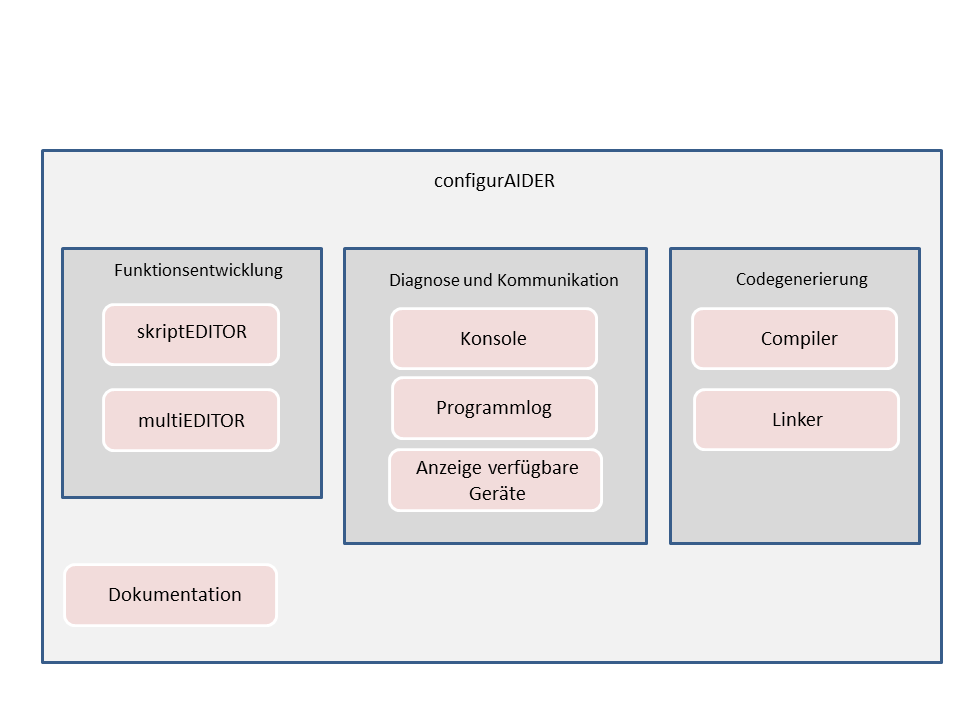
\includegraphics[width=\textwidth]{images/configurAIDER_Uebersicht.png}
	\caption{�bersicht configurAIDER}
	\label{fig:Uebersicht}
\end{figure}


\section{Elemente des configurAIDER}

\subsection{Rahmenfenster}
Der configurAIDER besteht aus einem Rahmenfenster, in das weitere Fenster eingebettet werden k�nnen. Das Rahmenfenster besitzt im oberen Fensterbereich eine Men�leiste in horizontaler Ausrichtung und ist in einem Hintergrund gehalten, der Firmenlogo und -farbe zeigt. Die Men�eintr�ge �ndern sind dynamisch in Abh�ngigkeit der vom Benutzer ge�ffneten Fenster. Beim Start des confiurAIDERs ist das Fenster "`Verf�gbare Ger�te"' standardm��ig in das Rahmenfenster eingebettet. Eingebettete Fenster k�nnen nicht �ber die Grenzen des Rahmenfensters hinausgezogen werden. 

%\begin{figure}[!htbp]
	%\centering
		%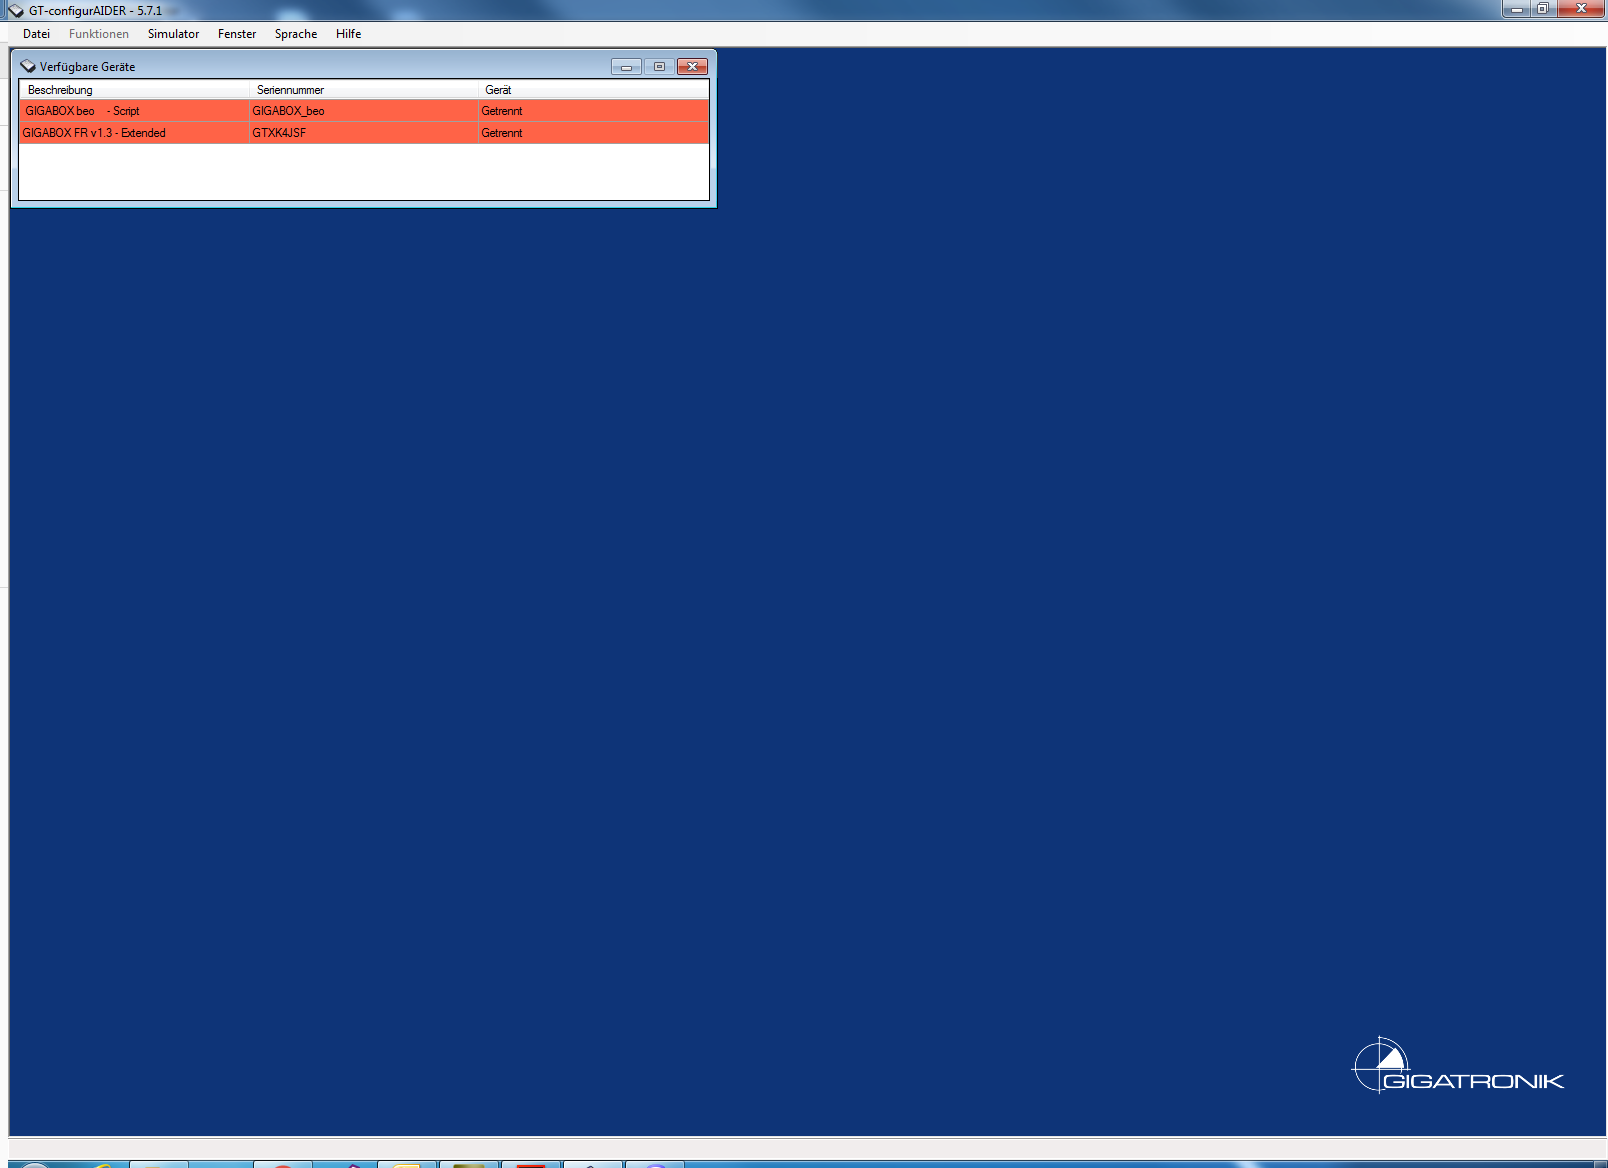
\includegraphics[width=\textwidth]{images/Rahmenfenster.png}
	%\caption{Rahmenfenster configurAIDER}
	%\label{fig:Rahmenfenster}
%\end{figure}



\subsection{Fenster "`Verf�gbare Ger�te"'}

Im Fenster "`Verf�gbare Ger�te"' werden alle GIGABOXen angezeigt, die an der USB-Schnittstelle des PC angeschlossen sind. Es wird der Modellname, die Seriennummer und der Verbindungsstatus von GIGABOXen ausgegeben, die am PC erkannt wurden. �ber dieses Fenster kann eine GIGABOX angew�hlt werden, mit der eine Kommunikation gestartet werden soll.  
Wenn keine reale GIGABOX zur Verf�gung steht, kann eine GIGABOX simuliert werden. 
Die Auswahl eines zu simulierenden Ger�tes erfolgt �ber ein eigenes Dialogfenster "`Simuliertes Ger�t"' (siehe Abbildung \ref{fig:SimuliertesGer�t}). 
 

\begin{figure}[!htbp]
	\centering
		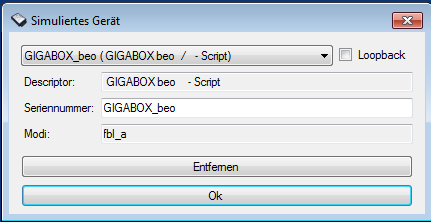
\includegraphics[width=\textwidth]{images/SimuliertesGeraet.png}
	\caption{Fenster "`Simuliertes Ger�t"'}
	\label{fig:SimuliertesGer�t}
\end{figure}

Die simulierte GIGABOX wird wie eine reale GIGABOX gelistet. 

Nach der Anwahl eines GIGABOX-Modelles wird versucht, eine Verbindung zu dem Ger�t herzustellen (wird das tats�chlich hardwarem��ig versucht oder ist die Anzeige nur dazu da, dem Benutzer zu signalisieren, welches Ger�t er konfiguriert). Bei erfolgreicher Verbindungsherstellung wird das Ger�t gr�n hinterlegt und es �ffnet sich ein Fenster zur Editorauswahl. Dort kann ausgew�hlt werden, ob die Konsole, der scriptEDITOR oder der multiEDITOR ge�ffnet werden soll. Bei einigen GIGABOX-Modellen steht kein multiEDITOR zur Verf�gung. 

\begin{figure}[!htbp]
	\centering
		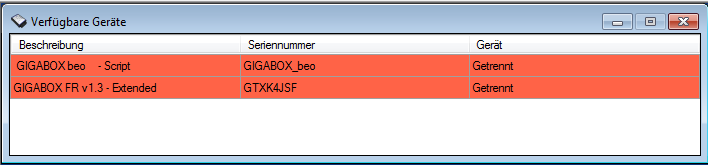
\includegraphics[width=\textwidth]{images/VerfuegbareGeraete.png}
	\caption{Fenster "`Verf�gbare Ger�te"'}
	\label{fig:Verf�gbareGer�te}
\end{figure}

\subsection{Fenster "`Konsole"'}

Die Konsole besteht aus einer Textbox zur Eingabe von Befehlen und einer Textbox zur Ausgabe von Informationen. Sie erm�glicht Kommunikation mit einer GIGABOX. Die Konsole kann z.B eingesetzt werden zur Abfrage von Diagnoseinformationen und um einen Reset zu veranlassen.  

�ber die Schaltfl�chen "`Folgen"' und "`Terminal"' kann gew�hlt werden, wie die Textein- und ausgabe erfolgen soll. Wenn "`Folgen"' ausgew�hlt wird, erfolgt die Texteingabe in einem von der Textausgabe getrennten Fenster. Wenn "`Terminal"' ausgew�hlt wird, erfolgt die Textein- und ausgabe in einem gemeinsamen Fenster. 



\begin{figure}[!htbp]
	\centering
		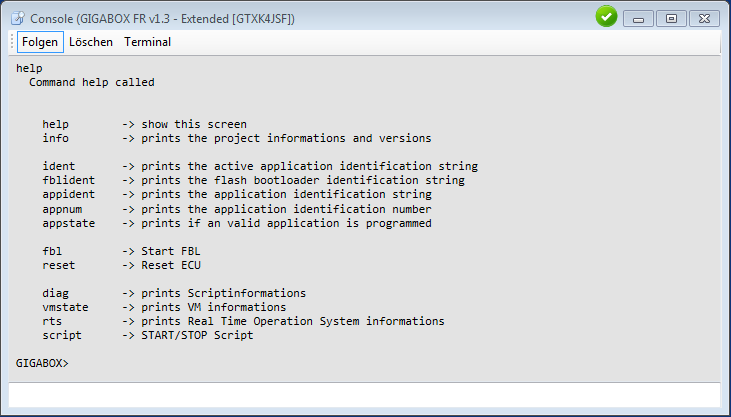
\includegraphics[width=\textwidth]{images/Konsole.png}
	\caption{Fenster "`Konsole"'}
	\label{fig:Konsole}
\end{figure}


\subsection{Fenster "`Programmlog"'}

Das "`Programmlog"'-Fenster besteht aus einer Textbox, �ber die tabellarisch Erfolgs- und Fehlermeldungen �ber die ausgef�hrten Aktionen des configurAIDERs ausgegeben werden.

\begin{figure}[!htbp]
	\centering
		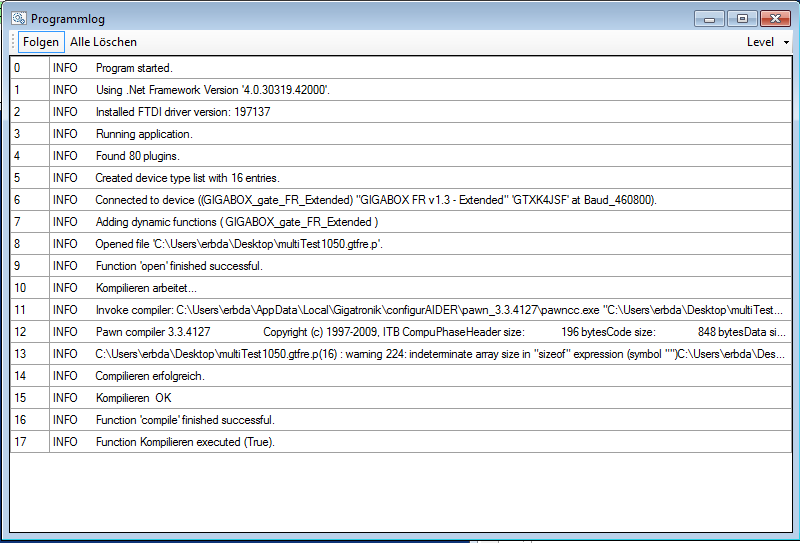
\includegraphics[width=\textwidth]{images/Programmlog.png}
	\caption{Fenster "`Programmlog"'}
	\label{fig:Programmlog}
\end{figure}


\subsection{Fenster "`scriptEDITOR"'}

Der scriptEDITOR ist ein Texteditor zum Erstellen und Editieren von Funktionen in PAWN. Um den scriptEDITOR aufzurufen, muss zuerst eine Verbindung zu einer realen oder simulierten GIGABOX hergestellt werden �ber das Fenster "`Verf�gbare Ger�te"'. Anschlie�end �ffnet sich automatisch ein Fenster zur Editorauswahl. Dort kann der scriptEDITOR angew�hlt werden. 
Mit dem scriptEDITOR erstellte Skriptdateien haben die Dateiendung .gt**.p. Die Sterne sind zu ersetzen mit einem K�rzel, das abh�ngig ist vom verbundenen GIGABOX-Modell. F�r die unterschiedlichen GIGABOX-Modelle werden also Skripte mit verschiedenen Dateiendungen erstellt, da die Modelle unterschiedliche Funktionen implementieren. Bsp: GIGABOX gate FR extended: .gtfre.p
GIGABOX gate XL: .gtxl.p
GIGABOX gate gateway: .gtfrg.p


In der obersten Fensterzeile ist eine Buttonleiste angeordnet mit den folgenden Buttons:
\begin{itemize}
	\item Neu: �ffnet ein neues Skript
	\item �ffnen: �ffnet ein vorhandenes Skript
	\item Speichern: Speichert das ge�ffnete Skript unter einem bereits festgelegt Dateinamen und Pfad
	\item Speichern unter: Speichert das ge�ffnete Skript unter einem anzugebenden Dateinamen und Pfad	
	\item Kompilieren: Interpreter erzeugt Bytecode aus dem PAWN-Quellcode  
	\item Herunterladen: Interpreter erzeugt Bytecode aus dem PAWN-Quellcode. Die PAWN-Skriptdatei wird als ZIP-Datei komprimiert. 
	Anschlie�end wird der Bytecode und das gezippte Skript auf die virtuelle Maschine der GIGABOX �bertragen.
	\item Heraufladen: Die als ZIP-Datei komprimierte Skriptdatei auf dem Steuerger�t wird auf den PC �bertragen, entzippt und im Texteditor ge�ffnet. 
	\item Reset: F�hrt einen Reset der GIGABOX durch
	\item Log: �ffnet Konsole	
			
\end{itemize}

\textcolor[rgb]{1,0,0}{Aufz�hlung der Buttons zu detailreich
}
Mittig ist der Texteditor angeordnet. Hier kann ein Skript angezeigt und bearbeitet werden. Es stehen bei der Entwicklung typische Unterst�tzungswerkzeuge wie Codefolding zur Verf�gung. \textcolor[rgb]{1,0,0}{(Aufz�hlung der unterst�tzenden Werkzeuge wie Autovervollst�ndigung etc.)}



Unten befindet sich ein Fenster zur Ausgabe von Fehlern, Warnungen und Erfolgsmeldungen.


\begin{figure}[!htbp]
	\centering
		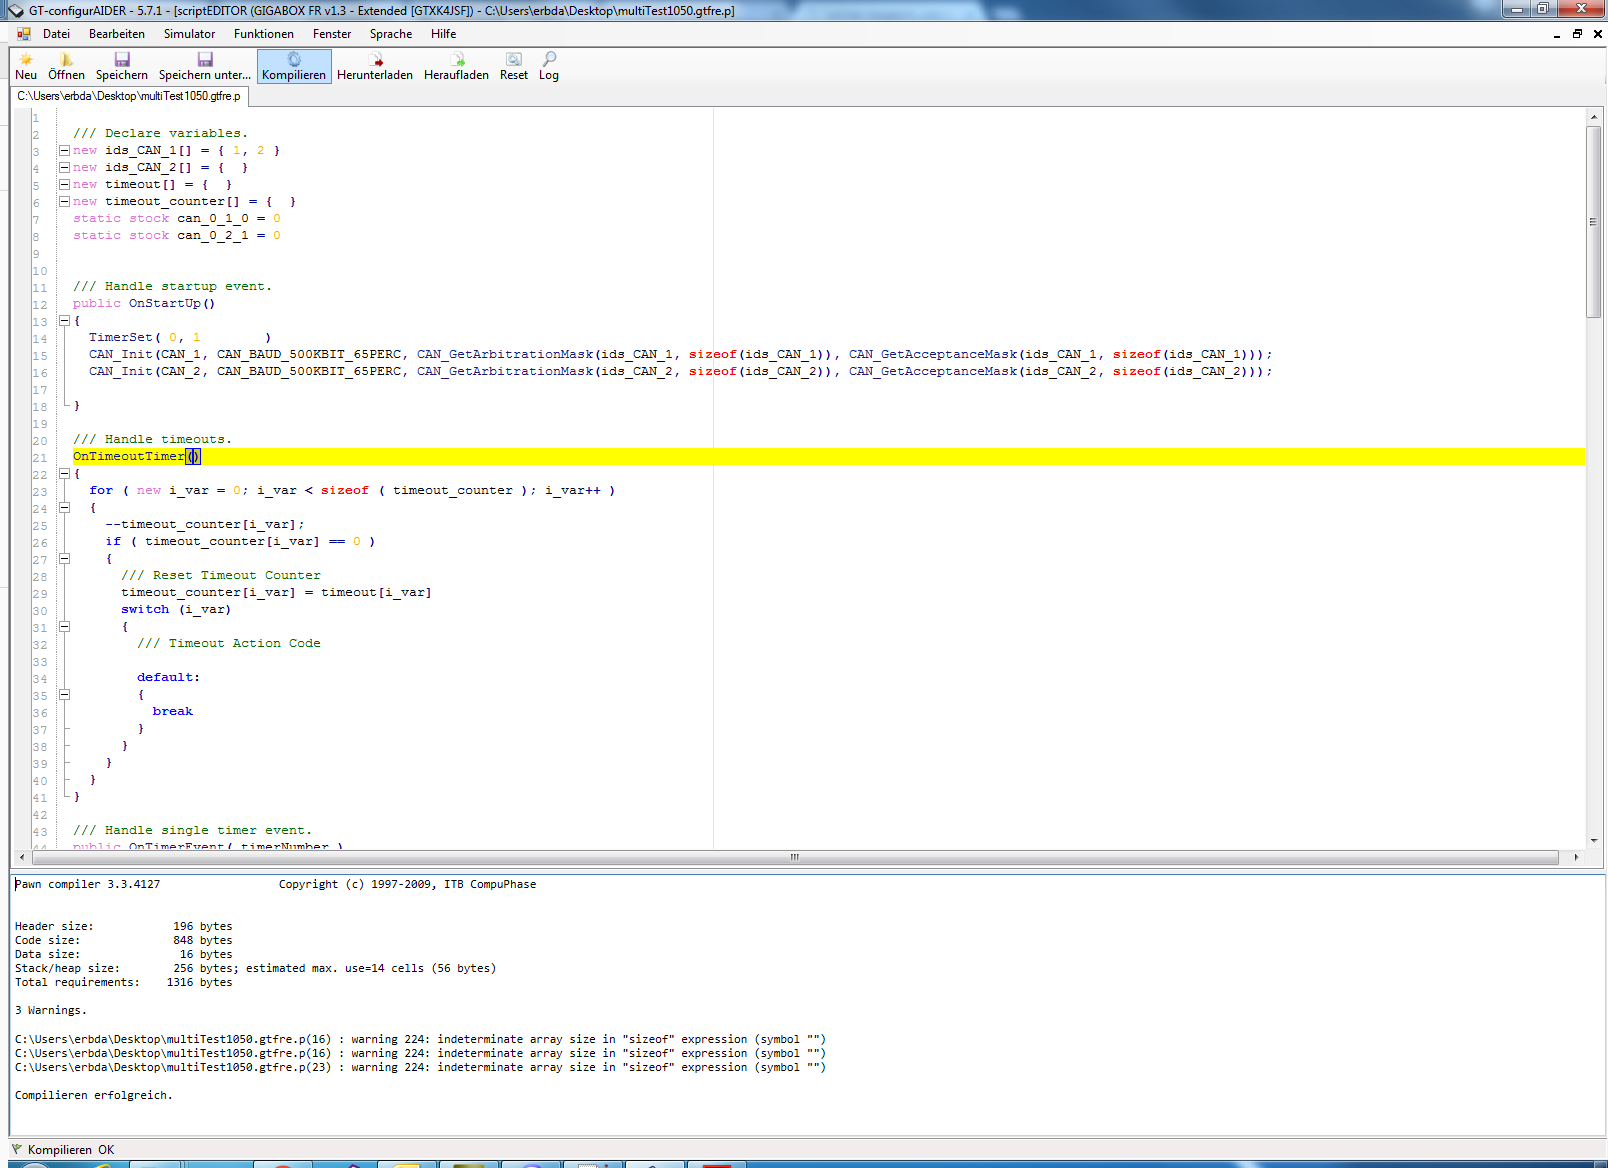
\includegraphics[width=\textwidth]{images/scriptEDITOR.png}
	\caption{Fenster "`scriptEDITOR"'}
	\label{fig:scriptEDITOR}
\end{figure}


\subsection{Fenster "`multiEDITOR"'}

Der "`multiEDITOR"' ist ein Editor zur Funktionskonfiguration mit WENN-DANN-Anweisungen in Tabellen. Er soll es Benutzern mit geringer Programmiererfahrung erm�glichen, einfache Funktionen f�r die GIGABOX zu entwickeln. Aus den konfigurierten Funktionstabellen kann anschlie�end automatisch ein PAWN-Skript generiert werden. Das erstellte PAWN-Skript kann dann kompiliert und der Bytecode auf den Flash-Speicher der GIGABOX �bertragen werden. 

In der obersten Fensterzeile ist eine Buttonleiste angeordnet mit den folgenden Buttons:
\begin{itemize}
	\item Neu: �ffnet ein neues Skript
	\item �ffnen: �ffnet ein vorhandenes Skript
	\item Speichern: Speichert das ge�ffnete Skript unter einem bereits festgelegt Dateinamen und Pfad
	\item Speichern unter: Speichert das ge�ffnete Skript unter einem anzugebenden Dateinamen und Pfad
	\item Generieren: Aus den mittels Tabelle konfigurierten Funktionen wird ein PAWN-Skript generiert
	\item Kompilieren: Interpreter erzeugt Bytecode aus dem PAWN-Quellcode  
	\item Herunterladen: Aus den mittels Tabelle konfigurierten Funktionen wird ein PAWN-Skript generiert. Interpreter erzeugt Bytecode aus dem PAWN-Quellcode. Die PAWN-Skriptdatei wird als ZIP-Datei komprimiert. 
	Anschlie�end wird der Bytecode und das gezippte Skript auf die virtuelle Maschine der GIGABOX �bertragen.
	
	\item Heraufladen: Die als ZIP-Datei komprimierte Skriptdatei auf dem Steuerger�t wird auf den PC �bertragen und entzippt.
	PAWN-Code wird r�ckgewandelt in Tabelle mit WENN-DANN-SONST-Anweisungen. Die funktioniert nur, wenn der von der GIGABOX hochgeladenen Code urspr�nglich mithilfe des multiEDITORs erzeugt wurde. 
	\item DBC: Es k�nnen Vector-DBC Dateien oder AUTOSAR .arxml Dateien erstellt oder ge�ffnet werden. Dabei handelt es sich um Datenbanken, in denen CAN-Botschaften und Signale definiert sind
	\item Reset: F�hrt einen Reset der GIGABOX durch
	\item Log: �ffnet Konsole
\end{itemize}
	
\textcolor[rgb]{1,0,0}{Aufz�hlung der Buttons zu detailreich
}	
	
Unter der Buttonleiste befindet sich eine Tabelle, in der CAN-Botschaften und Signale erstellt und bearbeitet werden k�nnen. Botschaften und Signale, die aus Datenbank-Dateien (.dbc oder .arxml) geladen wurden, werden hier angezeigt.
	
Darunter befindet sich eine Tabelle zur Konfiguration von Funktionen mithilfe von WENN-DANN-SONST-Anweisungen. 

\begin{figure}[!htbp]
	\centering
		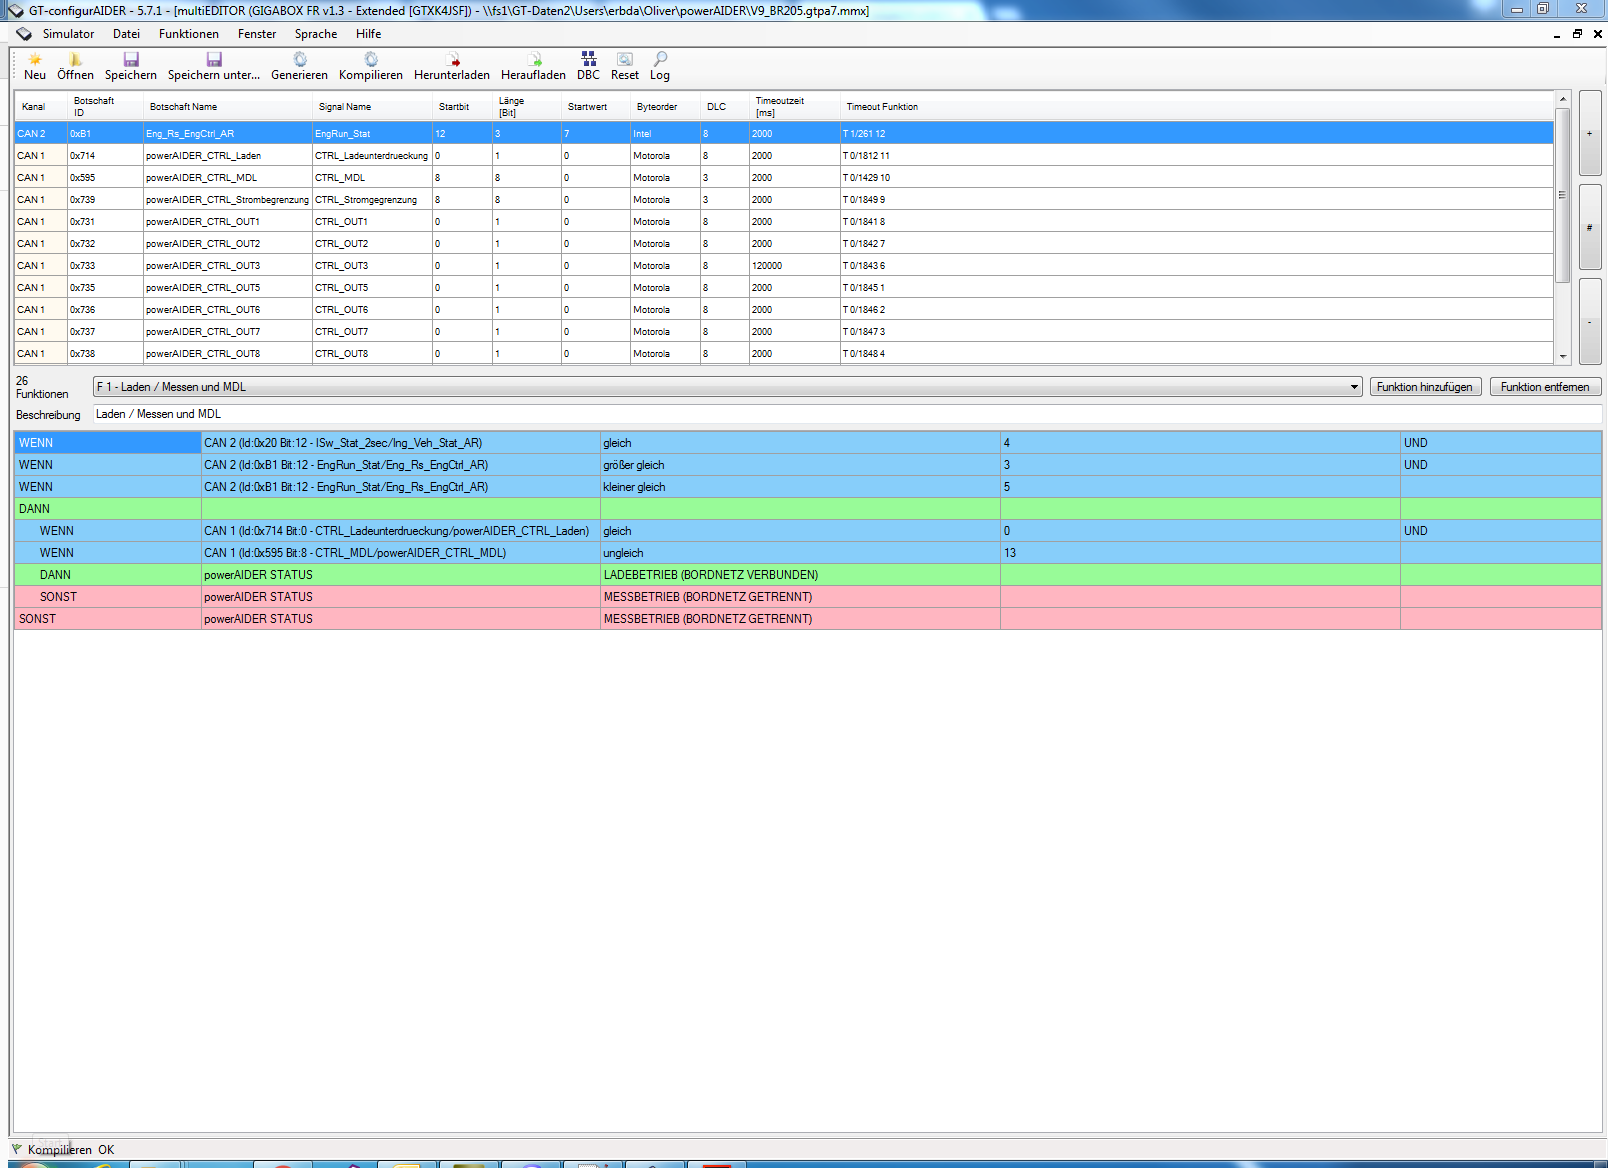
\includegraphics[width=\textwidth]{images/multiEDITOR.png}
	\caption{Fenster "`multiEDITOR"'}
	\label{fig:multiEDITOR}
\end{figure}



\section{Funktionalit�t} \label{sec:Funktionalit�t}

Abbildung \ref{fig:FunktionalitaetIst} gibt einen �berblick �ber die verf�gbaren Funktionen des configurAIDERs.

\begin{figure}[!htbp]
	\centering
		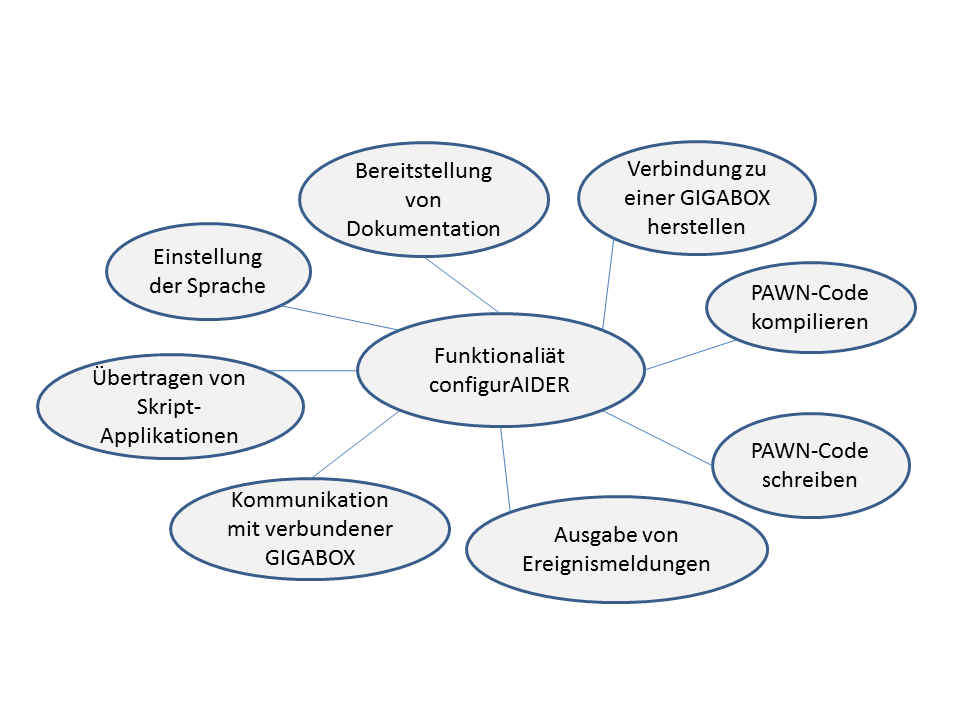
\includegraphics[width=\textwidth]{images/FunktionalitaetIst.png}
	\caption{�berblick Funktionen des configurAIDERs}
	\label{fig:FunktionalitaetIst}
\end{figure}

\subsection{Einstellung der Sprache}
Die Sprache der Fensterdialoge des configurAIDERs kann in der Men�leiste des Rahmenfenster unter dem Eintrag "`Sprache"' eingestellt werden. Es steht Deutsch und Englisch als Sprache zur Verf�gung. 
Nach der Sprache von Deutsch auf Englisch wird ein Dialog eingeblendet, dass die Sprach�nderung erst nach einem Neustart �bernommen wird. 
Nach ausgef�hrtem Neustart werden nicht alle Men�eintr�ge auf Englisch dargestellt. So werden beispielsweise im scriptEDITOR die Men�eintr�ge unter "`Edit"' weiterhin komplett in Deutsch dargestellt. Die Funktionstabellen im multiEDITOR werden auch weiterhin in Deutsch dargestellt.  

\subsection{Bereitstellung von Dokumentation zur GIGABOX, configurAIDER und PAWN}
�ber den Men�eintrag "`Hilfe"' k�nnen PDF-Dokumente zu den verschiedenen GIGABOX-Modellen, configurAIDER und zur Skriptsprache PAWN abgerufen werden. F�r den configurAIDER steht ein allgemeines Handbuch, Hinweise zur Installation und jeweils f�r scriptEDITOR und multiEDITOR ein eigenes Handbuch zur Verf�gung. Der Men�eintrag "`linEDITOR"' enth�lt nur einen ausgegrauten Eintrag.
Zu den GIGABOX-Modellen stehen Handb�cher, Flyer und Informationen zu Firmwareupdates zur Verf�gung. Die Dokumentationen werden nicht durchg�ngig f�r alle GIGABOX-Modelle zur Verf�gung gestellt. So wird f�r die GIGABOX gate xl kein Handbuch angeboten, f�r die GIGABOX gate powerAIDER kein Flyer.

\subsection{Verbindung zu einer GIGABOX herstellen}

GIGABOXEN, die an der USB-Schnittstelle des PCs erkannt werden sowie simulierte GIGABOXEN werden im Fenster "`Verf�gbare Ger�te"' (Abbildung \ref{fig:Verf�gbareGer�te}) gelistet. Hier kann die Verbindung zu einem Ger�t hergestellt werden. 
Falls keine reale GIGABOX zur Verf�gung steht, kann eine GIGABOX simuliert werden. 


Die verschiedenen Modelle besitzen unterschiedliche Hardwarefunktionen (unterschiedliche Anzahl von Ein-/Ausg�ngen, Bussysteme), die zu entwickelnden Funktionen m�ssen daran angepasst werden. Dem configurAIDER muss deshalb vor der Funktionsentwicklung bekannt sein, f�r welches Modell Code entwickelt werden soll.


Es wurden verschiedene Fehler entdeckt, die im Folgenden aufgelistet werden.

\begin{enumerate}
	\item Das Fenster "`Verf�gbare Ger�te"' wird vom Benutzer geschlossen. Bei einem Wiederaufruf des Fensters kann kein neues Ger�t mehr simuliert werden. L�sung: configurAIDER neu starten
	\item Im Fenster "`Verf�gbare Ger�te"' sind mehrere Ger�te gelistet. Bei dem Versuch, die Verbindung zu einem Ger�t herzustellen �ber Rechtsklick auf das Ger�t und "`Verbinden"', wird keine Verbindung zum angew�hlten Ger�t hergestellt sondern zum ersten Ger�t in der Liste. L�sung: Verbindung herstellen �ber Doppelklick auf Ger�t
	\item Die Simulation von Ger�ten schl�gt gelegentlich fehl, es wird �ber das Programmlog-Fenster ein Fehler ausgegeben (ERROR: Internal device table obscurred!) L�sung: Neuer Versuch der Herstellung einer Verbindung

\end{enumerate}


\subsection{PAWN-Code kompilieren}

Aus scriptEDITOR und multiEDITOR heraus kann mithilfe des Compilers PAWN-Code in Bytecode �bersetzt werden. Der erzeugte Bytecode kann auf der virtuellen Maschine der GIGABOX ausgef�hrt werden.


\subsection{PAWN-Code entwickeln}

	\subsubsection{PAWN-Skripte schreiben}

	PAWN-Skripte k�nnen im scriptEDITOR geschrieben werden. 
	Erstellte Skriptdateien besitzen die Dateiendung .gt**.p. 
	Die Sterne sind zu ersetzen mit einem K�rzel, das abh�ngig ist vom verbundenen GIGABOX-Modell.
F�r die unterschiedlichen GIGABOX-Modelle werden also
	Skripte mit verschiedenen Dateiendungen erstellt, da die Modelle unterschiedliche
	Funktionen implementieren. Bsp: GIGABOX gate FR extended: .gtfre.p
	GIGABOX gate XL: .gtxl.p GIGABOX gate gateway: .gtfrg.p
	
	Um den Benutzer bei der Codeentwicklung zu unterst�tzen, sind aus anderen IDEs bekannte Funktionen integriert. Einige ausgew�hlte Funktionen sind hier beispielhaft angef�hrt:

	\begin{itemize}
		\item Codeabschnitte sind auf- und zuklappbar
		\item Unterschiedliche Farbgebung (Anweisungen in blau, Kommentare in gr�n etc)
		\item Eventfunktionen sind als Rumpf vorimplementiert
		\item Markierung der Zeile, in der sich der Cursor aktuell befindet	
	\end{itemize}

	Im Vergleich zu weit verbreiteten IDEs wie Visual Studio ist der Umfang an unterst�tzenden Funktionen aber klein gehalten.







	\subsubsection{PAWN-Skripte aus Funktionstabellen generieren}

	Im multiEDITOR k�nnen tabellarisch Funktionen konfiguriert werden mit WENN-DANN-SONST-Anweisungen. Aus den konfigurierten Funktionstabellen kann anschlie�end automatisch
	ein PAWN-Skript generiert werden. Das erstellte PAWN-Skript kann
	dann kompiliert und der Bytecode auf den Flash-Speicher der GIGABOX �bertragen
	werden.
	
	F�r jede Funktion wird eine neue Tabelle erstellt. Jede Tabelle besteht mindestens aus 3 Zeilen mit den Anweisungen WENN, DANN und SONST. Es k�nnen mehrere WENN-Anweisungszeilen erstellt werden, die mit dem Bedingungsoperator UND oder ODER verkn�pft werden m�ssen. Au�erdem k�nnen mehrere DANN und SONST-Anweisungen erstellt werden, die jeweils miteinander �ber den UND-Operator verkn�pft werden.
	Unter jeweils jede DANN und SONST-Anweisung kann eine neue, untergeordnete  WENN-DANN-SONST-Anweisung eingef�gt werden. Damit sind verschachtelte Anweisungen m�glich. 

	In den Spalten der WENN-Anweisungszeile k�nnen digitale und analoge Eing�nge, digitale Ausg�nge sowie eingehende Busbotschaften auf definierte Werte gepr�ft werden. 
	Wenn die dort definierten Werte angenommen werden, wird die DANN-Anweisungenszeile ausgef�hrt. Hier k�nnen digitale Ausg�nge durchgeschaltet oder ausgeschaltet werden. Das Absetzen von Busbotschaften ist nicht m�glich.  

	Wenn die in der WENN-Anweisungszeile definierten Werte nicht angenommen werden, wird die SONST-Anweisungszeile ausgef�hrt. Auch hier k�nnen digitale Ausg�nge durchgeschaltet oder ausgeschaltet werden. 
	
	\textcolor[rgb]{1,0,0}{Bewertung}


\subsection{�bertragen von Skript-Applikationen}

Es kann eine Skript-Applikation auf die GIGABOX �bertragen werden. Die Skriptdatei wird als ZIP-Datei komprimiert und zusammen mit dem Bytecode auf den Flash-Speicher geschrieben. Wenn ein Skript mithilfe des multiEDITORs generiert wurde, wird zus�tzlich zu der Skriptdatei (.gt**.p) auch die multiEDITOR-Konfigurationsdatei (.gt**.mmx) \textcolor[rgb]{1,0,0}{(+.tmp -> was steht da drin?)} mit in die ZIP-Datei gepackt.

Ein auf der GIGABOX ausgef�hrtes Skript kann auch von der GIGABOX auf den PC geladen werden. Dabei wird die auf der GIGABOX gespeicherte ZIP-Datei auf den PC geladen, entpackt und im scriptEDITOR angezeigt. Wenn das Skript mit dem multiEDITOR erzeugt wurde, liegt der ZIP-Datei zus�tzlich die multiEDITOR-Konfigurationsdatei (.gt**.mmx) bei und kann folglich auch im multiEDITOR ge�ffnet werden.



\subsection{Kommunikaton mit verbundener GIGABOX}

�ber die Konsole k�nnen Befehle an eine reale GIGABOX gesendet werden, z.B. Befehl zum Reset, Aufrufen des Bootloaders. 
Dort k�nnen auch Informationen der GIGABOX abgerufen und ausgeben werden, z.B. Diagnoseinformationen �ber Bussysteme oder Timer.

Wenn die Schaltfl�che "`Terminal"' aktiviert ist, kann eine erfolgte Texteingabe nicht mehr korrigiert werden. Bei deaktivierter Schaltfl�che ist die Korrektur m�glich. 

\subsection{Ausgabe von Ereignismeldungen}

Es kann �ber das Programmlog-Fenster nachverfolgt werden, welche Aktionen vom configurAIDER durchgef�hrt wurden. Wichtige Erfolgs- und Fehlermeldungen werden dort ausgegeben. Bsp: Erfolgreich kompiliert.






\subsection{Ergebnis}




	\chapter{Evaluation}

\section{Funktionalit�t und Usability des Ist-Zustands}

Es sollen die Funktionen des configurAIDERs bewertet werden hinsichtlich Umfang, Umsetzung und Fehlerzust�nden. Zus�tzlich soll die Usability nach EN ISO 9241-110 (siehe Abschnitt \ref{sec:Qualit�tskriterienSW}) bewertet werden.

\subsection{Einstellung der Sprache}
Es kann Deutsch und Englisch als Sprache eingestellt werden. Hier w�re zu �berlegen, ob noch weitere Spracheinstellungen zur Verf�gung gestellt werden sollten, falls es eine gr��ere Anzahl an Benutzern aus nicht deutsch- oder englischsprachigen L�ndern gibt.
Die englische Spracheinstellung ist nicht konsistent umgesetzt, hier sollte darauf geachtet werden, dass durchg�ngig alle Bedienelemente englisch beschriftet werden.  

\subsection{Bereitstellung von Dokumentation zur GIGABOX, configurAIDER und PAWN}
�ber den Men�eintrag "`Hilfe"' k�nnen PDF-Dokumente zu den verschiedenen GIGABOX-Modellen, configurAIDER und zur Skriptsprache PAWN abgerufen werden. F�r den configurAIDER steht ein allgemeines Handbuch, Hinweise zur Installation und jeweils f�r scriptEDITOR und multiEDITOR ein eigenes Handbuch zur Verf�gung. Hier ist zu kritisieren, dass der Men�eintrag "`linEDITOR"' nur einen ausgegrauten Eintrag enth�lt und somit unn�tig ist.
Zu den GIGABOX-Modellen stehen Handb�cher, Flyer und Informationen zu Firmwareupdates zur Verf�gung. Leider werden die Dokumentationen nicht durchg�ngig f�r alle GIGABOX-Modelle zur Verf�gung gestellt. So wird f�r die GIGABOX gate xl kein Handbuch angeboten, f�r die GIGABOX gate powerAIDER kein Flyer.

\subsection{Verbindung zu einer GIGABOX herstellen}


F�r den Benutzer ist nicht zu unterscheiden, ob ein Ger�t in der Liste real oder simuliert ist. 
Simulierte Ger�te werden in der Liste nicht hervorgehoben oder markiert. Die gew�nschte Aufgabenangemessenheit ist f�r dieses Fenster damit nicht gegeben, da der Benutzer die Auswahl einer GIGABOX nicht effizient erledigen kann. 

Die Auswahl eines zu simulierenden Ger�tes erfolgt �ber ein eigenes Dialogfenster "`Simuliertes Ger�t"' (siehe Abbildung \ref{fig:SimuliertesGer�t}). 
F�r den Benutzer ist in diesem Dialog nicht ersichtlich, was die Checkbox "`Loopback"' bewirkt. Die Selbsterkl�rungsf�higkeit des Dialogs ist nicht ausreichend. 

Bei der Auswahl eines zu simulierenden Ger�tes im Fenster "`Simuliertes Ger�t"' wird das angew�hlte Ger�t der Liste  im Fenster "`Verf�gbare Ger�te"' hinzugef�gt, bevor die Auswahl mit "`Ok"' best�tigt wird. Diese Reaktion entspricht nicht den �blichen, dem Benutzer bekannten Konventionen von Software und ist damit nicht erwartungskonform.



Aufgrund von diverse Fehlerzust�nden, die beobachtet wurden, kann die Verbindung zu einem Ger�t nicht zuverl�ssig und fehlerfrei hergestellt werden. Das Tool produziert Ergebnisse, die vom Benutzer so nicht erwartet werden und erfordert l�stiges Neustarten des Programmes. 





\subsection{PAWN-Code kompilieren}

Die Kompilierung funktioniert ohne Probleme.


\subsection{PAWN-Code entwickeln}

	\subsubsection{PAWN-Skripte schreiben}
	
	Keine M�glichkeit, letzte Aktion r�ckg�ngig zu machen -> schlechte Steuerbarkeit
	
Keine Erkennung von Syntaxfehlern -> schlechte Selbstbeschreibungsf�higkeit

Buttons Herunterladen/Heraufladen sind missverst�ndlich -> schlechte Selbstbeschreibungsf
�higkeit

Nur ein Skript kann ge�ffnet werden, nicht mehrere gleichzeitig -> Aufgabenangemessenheit

Autovervollst�ndigung nur teilweise umgesetzt -> Aufgabenangemessenheit

Codebl�cke k�nnen nicht auskommentiert werden �ber Buttons/Tastenkombination
-> Aufgabenangemessenheit



	
	Die Buttons "`Herunterladen"' und "`Heraufladen"' in der oberen Buttonleiste sind nicht klar verst�ndlich benannt. Dem Benutzer wird nicht klar, in welche Richtung der Datenaustausch erfolgt. Der Button "`Log"' �ffnet die Konsole, die Erwartung w�re, dass sich das Programmlog-Fenster �ffnet. Die Selbstbeschreibungsf�higkeit und Erwartungskonformit�t der Buttonleiste ist negativ zu bewerten.





	\subsubsection{PAWN-Skripte aus Funktionstabellen generieren}

	Im Signaleditor ist Bit/CAN-Bit Unterschied nicht klar ersichtlich -> Selbstbeschreibungsf�higkeit
	
	Es k�nnen keine CAN-Nachrichten gesendet werden -> eingeschr�nkte Funktionalit�t
	
	Keine Reaktion auf LIN-Nachrichten m�glich/ kein Senden von LIN-Nachrichten m�glich
	
	Keine M�glichkeit, SWITCH CASE-Anweisung einzuf�gen. Deshalb m�ssen verschachtelte WENN DANN-Anweisungen erstellt werden, die 	schnell un�bersichtlich werden
	
	Es ist nicht ersichtlich, dass �ber den DBC-Button auf .arxml-Dateien geladen werden k�nnen
	
Bei Klick auf DBC-Button �ffnet sich Fenster zum Laden von .dbc und .armxl-Dateien. In diesem Fenster befindet sich eine Tabelle zur Anzeige der geladenen Signale. Bei Anwahl einer .dbc-Datei bleibt die Tabelle allerdings leer. Die im ausgew�hlten DBC definierten Signale werden dort nicht angezeigt

\subsection{�bertragen von Skript-Applikationen}

Das �bertragen 	von Skript-Applikationen funktioniert ohne Probleme.

\subsection{Kommunikaton mit verbundener GIGABOX}

Wenn die Schaltfl�che "`Terminal"' aktiviert ist, kann eine erfolgte Texteingabe nicht mehr mit der R�cktaste korrigiert werden. Bei deaktivierter Schaltfl�che ist die Korrektur m�glich. Die Konsole mangelt es folglich an Fehlertolernaz, was einer schlechten Usability entspricht. 

\subsection{Ausgabe von Ereignismeldungen des configurAIDERs}

Die Ausgabe von Ereignismeldungen �ber das Programmlog-Fenster ist zufriedenstellend.

\section{Differenz zwischen Anforderungen und Ist-Zustand}

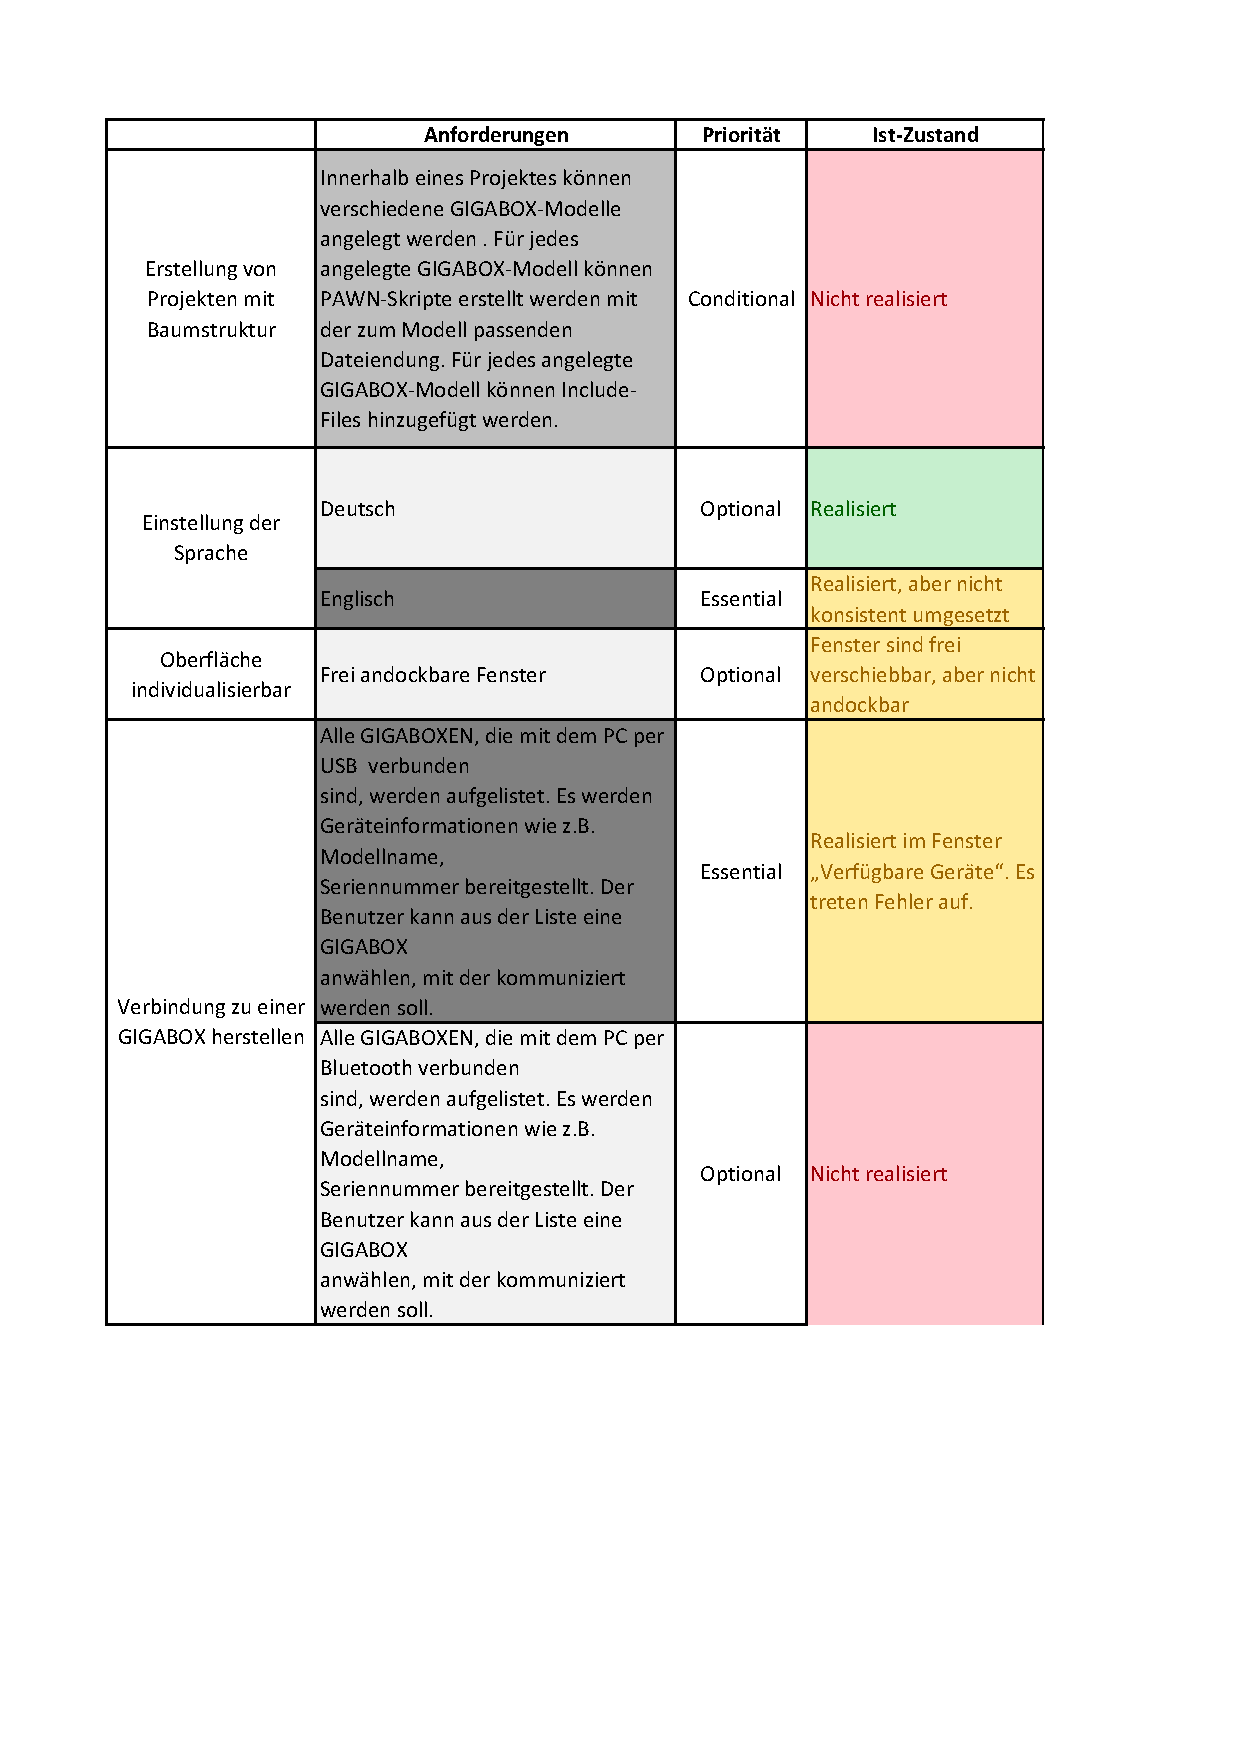
\includepdf[pages=-, landscape=false]{images/SollIstVergleich}




\section{Quellcode des configurAIDERs}

\colorbox[rgb]{1,0,0}{Was wurde mit WinForms gemacht, was mit WPF?}

Entstand aus mehreren studentischen Arbeiten

\colorbox[rgb]{1,0,0}{Diagramm mit bestehender Architektur erstellen}

\section{Ergebnis}


	\chapter{Konzeption}

\section{�bersicht}

Ziel des Kapitels ist es, Konzepte aufzuzeigen, wie die in der Anforderungsanalyse erarbeiteten Anforderungen umgesetzt werden k�nnen.

\section{Erweiterung des bestehenden configurAIDERs um neue Features}

Der bestehende Code des configurAIDERs wird erweitert um neue Features, die bei der Bewertung der Anforderungen in Abschnitt \ref{sec:BewertungAnforderungen} mit (+) oder (++) bewertet wurden. Die an bereits bestehenden Features in Abschnitt \ref{sec:Funktionalit�t} kritisierten Punkte sollen verbessert werden.

Neue Funktionen:
\begin{itemize}
	\item Projektverwaltung: Es k�nnen Projekte angelegt werden, in denen unterschiedliche Modelle der GIGABOX projektiert sind und die zugeh�rigen Skripte+Include-Files
	\item Texteditor wird erweitert um:
	
	\begin{enumerate}
		\item M�glichkeit, letzte Schritte r�ckg�ngig zu machen
		\item Anzeige aller implementierten Funktionen zur Navigation im Skript
		\item Bei der Codeentwicklung unterst�tzende Funktionen
		\item Routing-Editor
	\end{enumerate}
	
	\item Frei andockbare Fenster
	\item Steuern und Beobachten von DIN, AIN, DOUT, SWITCH
	
\end{itemize}

Vorteil: 

\begin{itemize}
	\item Das Tool erh�lt damit einen erh�hten Funktionsumfang, als wichtig bewertete funktionale Anforderungen k�nnen umgesetzt werden.
	
\end{itemize} 

Nachteil: 
\begin{itemize}
	\item Nichtfunktionale Anforderungen wie Qualit�tskriterien an Software nach ISO9126 (Wartbarkeit, Usability, Effizienz, �bertragbarkeit, Zuverl�ssigkeit) k�nnen nicht erf�llt werden, sondern werden sich verschlechtern durch eine weitere Funktionserweiterung des Tools
	
	
	\item Viel Einarbeitung in bestehenden Code n�tig

\end{itemize}


\section{Neuentwicklung des configurAIDERs} 

Das Tool wird von Grund auf neu entwickelt. Es sollen die funktionalen und nichtfunktionalen Anforderungen aus Kapitel \ref{chp:Anforderungsanalyse} umgesetzt werden. Im Rahmen dieser Arbeit sollen vorerst nur die wichtigsten funktionalen Anforderungen umgesetzt werden (mit ++ bewertet). Allerdings sollen alle nichtfunktionalen Anforderungen erf�llt werden.

Funktionen:

\begin{itemize}
\item Projektverwaltung: Es k�nnen Projekte angelegt werden, in denen unterschiedliche Modelle der GIGABOX projektiert sind und die zugeh�rigen Skripte+Include-Files
\item Texteditor 
	\begin{itemize}
		\item mehrere Skripte lassen sich parallel �ber Tabs �ffnen
		\item Copy/Paste
		\item Suchen/Ersetzen
		\item M�glichkeit, letzte Schritte r�ckg�ngig zu machen
		\item Bei der Codeentwicklung unterst�tzende Funktionen. Ziel: Schnelles
und effektives Schreiben von fehlerfreiem Code
	\end{itemize}
	
\item Erkennung von GIGABOXEN, die mit dem PC verbunden sind
\item PAWN-Compiler
\item Beschreiben/Auslesen des Flash-Speichers der GIGABOX
\item Konsole
\item Bereitstellen von Dokus

\end{itemize}


Vorteil:
\begin{itemize}
	\item Tool wird einfacher erweiterbar als bisheriger Stand. Dies erm�glicht es, zuk�nftig einfacher neue Features zu integrieren.
	\item Besser wartbar: Bugs k�nnen in Zukunft besser behoben werden, da Verhalten des neuen Codes besser bekannt ist
	\item Usability kann verbessert werden
	\item Tool konsistent mit WPF realisiert unter aktueller .NET Version 4.6
	\item Keine lange Einarbeitung in alten Code n�tig
\end{itemize}

Nachteil:
\begin{itemize}
	\item In Entwurf der neuen Softwarearchitektur muss Zeit investiert werden
	\item Tool bietet keinen direkten Mehrwert in Form von h�herem Funktionsumfang 
	\item Insgesamt h�herer Aufwand um die gestellten funktionalen Anforderungen zu erreichen
\end{itemize}


	\chapter{Design}

\section{�berblick}

In Kapitel \ref{chp:Evaluation} wurde entschieden, eine Neuentwicklung des configurAIDERs weiter zu verfolgen. Hierzu muss die Benutzeroberfl�che neu entworfen werden, eine neue Software-Architektur entwickelt werden und anschlie�end eine Umsetzung in Programmcode erfolgen. Dieses Kapitel besch�ftigt sich mit dem Entwurf einer neuen Benutzeroberfl�che und dem Herleiten einer neuen Softwarearchitektur. 

\section{Entwurf der Benutzeroberfl�che} \label{sec:EntwurfUI}

Die Benutzeroberfl�che soll so entworfen werden, dass die in der Anforderungsanalyse erarbeiteten Use Cases erf�llt werden k�nnen.
Zus�tzlich sollen die in Abschnitt \ref{sec:Qualit�tskriterienSW} definierten Grunds�tze der Dialoggestaltung aus ISO ISO/IEC 25010 beachtet werden.

Abbildung \ref{fig:Mockup} zeigt ein Mockup der Benutzeroberfl�che, das diese Kriterien erf�llt.

\begin{figure}[!htbp]
	\centering
		\includegraphics[width=\textwidth]{images/configurAIDER_Mockup.png}
	\caption{Mockup der Benutzeroberfl�che des configurAIDERs}
	\label{fig:Mockup}
\end{figure}

Die Hauptelemente der Benutzeroberfl�che sind ein Texteditor, ein Projektexplorer, eine Ger�teliste sowie eine Konsole. 
Zur Bedienung dieser Hauptelemente verf�gt die GUI �ber eine Men�leiste, eine Toolbar mit Buttons sowie �ber Kontextmen�s.
Die Men�leiste stellt Funktionen bereit, die im jeweiligen Bedienungskontext zur Verf�gung stehen. 
Den Zugriff auf h�ufig ben�tigte Funktionen soll eine Toolbar erm�glichen.

Die Toolbar enth�lt folgende Buttons:

\begin{itemize}
	\item Neues Projekt erstellen
	\item Projekt �ffnen
	\item Datei �ffnen
	\item Datei speichern
	\item Datei speichern unter
	\item Datei kompilieren
	\item Datei flashen
\end{itemize}

Die vier GUI-Hauptelemente werden innerhalb eines einzelnen Programmfensters dargestellt, um dem Benutzer einen zentralen Zugriff auf alle zur Verf�gung stehenden Funktionen zu erm�glichen. 

Als zentrales Element ist in der Mitte des Fensters der Texteditor angeordnet, da f�r die Anzeige von Quellcode viel Platz beansprucht wird. Um innerhalb von gr��eren Programmskripten zu navigieren, muss der Texteditor scrollbar sein.	

Die Konsole ist unterhalb des Texteditors ausgerichtet, da ein breites Eingabefeld f�r Befehle ben�tigt wird. 
Sie besteht aus einer Eingabezeile, die als oberstes Steuerelement angeordnet ist sowie aus einem darunterliegenden Ausgabefeld.
Da in vertikale Richtung wenig Platz zur Verf�gung steht, muss die Textausgabe der Konsole scrollbar sein. 

Der Projektexplorer kann ein Projekt darstellen, das eine Baumstruktur aus Ordnern und Pawn-Dateien beinhaltet. 
Das Projekt repr�sentiert das Wurzelelement des Baumes und stellt Ebene 1 der Struktur dar. 
Die Kindelemente des Projektes k�nnen Ordner sowie Pawn-Dateien sein, sie repr�sentieren Ebene 2 der Struktur.
Ordner wiederum k�nnen nur Pawn-Dateien als Kindelemente enthalten, somit ist die Baumstruktur auf drei Ebenen beschr�nkt. 
Das Hinzuf�gen von Kindelementen soll �ber ein Kontextmen� des Elternelementes m�glich sein.

In der Ger�teliste werden �ber USB verbundene GIGABOX FD-Ger�te untereinander aufgelistet. Zu jedem Ger�t wird eine Checkbox dargestellt, mit der eine GIGABOX als Zielger�t ausgew�hlt werden kann. 
Wurde ein Zielger�t festgelegt, steht im configurAIDER die Flash-Funktion zur Verf�gung und in die Konsole eingegebene Befehl werden an das Zielger�t gesendet.


(Vereinzelt Designbegr�ndung nach ISO einf�gen)

Erl�uterung des Entwurfes mit Bezugnahme auf ISO, die gute Usability definiert

	
\section{Entwurf der Softwarearchitektur}

\textit{"`The software architecture of a program or computing system is the structure or structures of the system, which comprises software components, the externally visible properties of those components and the relationship among them."'} \cite{DefSWArchitektur}

Nach dieser in der Literatur oft zitierten Definition legt die Softwarearchitektur die Komponenten eines Systems fest, beschreibt deren wesentliche, von au�en sichtbare Merkmale und charakterisiert die Beziehungen dieser Komponenten. Sie beschreibt den statischen Aufbau einer Software im Sinne eines Bauplans und den dynamischen Ablauf einer Software im Sinne eines Ablaufplans. 

Die in diesem Kapitel vorgestellte Software-Architektur des configurAIDERs wurde entworfen auf Basis der funktionalen und nichtfunktionalen Anforderungen an Software in Kapitel \ref{chp:Anforderungsanalyse}. Wie im vorigen Kapitel "`Konzeption"' erl�utert, werden nur Funktionen umgesetzt, die als "`Essential"' oder "`Conditional"' priorisiert wurden.

Die Softwarearchitektur wird aus verschiedenen Sichten dargestellt, da eine einzelne Darstellung die Komplexit�t eines Systems nicht wiedergeben kann. 
Jede Sicht zeigt das System detailliert aus einer bestimmten Perspektive. Details, die f�r eine Sicht nicht von Bedeutung sind, werden vernachl�ssigt. Es werden drei Arten von Sichten verwendet: die Kontextabgrenzung, die Bausteinsicht und die Laufzeitsicht.
Die verschiedenen Sichten werden in UML-Diagrammen dargestellt. F�r die Darstellung der Kontextabgrenzung wird ein Deployment Diagramm verwendet, f�r die Bausteinsicht Klassendiagramme und f�r die Laufzeitsicht Sequenzdiagramme. 
Die Einteilung in diese Sichtarten wird in Buch \cite{EffSWArchitektur} empfohlen.  

Zur Verdeutlichung kann man sich die Erstellung einer Geb�udearchitektur anschauen, bei der �hnlich vorgegangen wird.
 Das Geb�ude wird aus verschiedenen Sichten dargestellt, z. B. Grundriss, Geb�udeplan und Elektroplan. Jede Sicht konzentriert sich auf die Darstellung von Details, die f�r diese Sicht wichtig sind und vernachl�ssigt daf�r anderes, um die Darstellung nicht zu �berladen.

Quelle: \cite{EffSWArchitektur}

\subsection{Model-View-ViewModel-Pattern (MVVM-Pattern)}	\label{sec:MVVM}

Das Model-View-ViewModel-Pattern (MVVM) ist ein Software-Architekturmuster. Das Muster basiert auf der Idee des Model-View-Controller-Patterns (MVC), die Verantwortlichkeiten f�r Darstellung und Layout der Benutzeroberfl�che von der Logik der Benutzeroberfl�che zu trennen. Das MVVM-Pattern verwendet drei Komponenten, die jeweils unterschiedliche, voneinander getrennte Verantwortlichkeiten besitzen. Diese drei Komponenten sind die View, das Model und das ViewModel.

Die View ist zust�ndig f�r Aussehen und Struktur der Elemente der Benutzeroberfl�che. In WPF wird die View in einer XAML-Datei beschrieben. Jede XAML-Datei ist untrennbar mit einer Codebehind-Datei gekoppelt, in der UI-Logik implementiert werden kann. Nach dem MVVM-Pattern soll im Codebehind keine Logik implementiert werden, die au�erhalb der Verantwortlichkeiten der View liegt. 

Das Model enth�lt die Daten, die dem Benutzer �ber die View angezeigt werden und von diesem bearbeitet werden k�nnen. Hier wird auch eine Validierung der eingegebenen Daten vorgenommen.

Das ViewModel stellt das Bindeglied zwischen View und Model dar. Hier wird die UI-Logik implementiert. 
Die Daten des Models werden im ViewModel manipuliert, um sie in geeigneter Weise �ber die View darstellen zu k�nnen. View und ViewModel werden nach dem MVVM-Pattern ausschlie�lich mithilfe von Data Bindings und Commands gekoppelt.
Data Binding erm�glich der View, sich an Properties des ViewModels zu binden und damit auf ben�tigte Daten zugreifen zu k�nnen.
Beispielsweise kann ein Texteingabefeld der View �ber Data Binding an eine \texttt{string}-Property im ViewModel gebunden werden. Im ViewModel steht dann der Inhalt der Textbox als \texttt{string} zur Verf�gung, kann dort weiterverarbeitet und anschlie�end im Model gespeichert werden.
Commands werden eingesetzt, um auf Benutzeraktionen wie einen Klick auf einen Button reagieren zu k�nnen. Jedes in der View definierte UI-Element, das das Interface \texttt{ICommandSource} implementiert, l�st bei einer definierten Aktion ein Command aus.
�ber Data Binding kann auf ein Property vom Typ \texttt{ICommand} im ViewModel gebunden werden. Dort wird die \emph{Execute}-Methode, die im \texttt{ICommand}-Interface enthalten ist, aufgerufen. In der \emph{Execute}-Methode wird schlie�lich die Logik definiert, die die Benutzeraktion ausl�sen soll.




�ndern sich im Model oder im ViewModel Daten, die �ber Data Binding an die View gebunden sind, muss die View �ber �nderungen informiert werden. Sie kann dann von dem Property, das die ge�nderten Daten bereitstellt, die Daten neu abfragen und die aktualisierten Daten auf der Benutzeroberfl�che ausgeben. Ein solcher Benachrichtigungsmechanismus kann realisiert werden, indem alle Model- und ViewModel-Klassen das Interface \texttt{INotifyPropertyChanged} implementieren. Jede dieser Klassen muss dann ein Event deklarieren, das ein Delegat vom Typ \texttt{PropertyChangedEventHandler} verwendet. Wird ein Property neu gesetzt, wird das Event ausgel�st und als Folge davon die View dar�ber benachrichtigt, in welchem Property �nderungen vorgenommen wurden.

Abbildung \ref{fig:MVVMPrinciple} zeigt beschriebene Prinzip aus Data Binding, Commands und Benachrichtigungen.

Quelle: \cite{MSMVVM}, \cite{WPF}

\begin{figure}[!htbp]
	\centering
		\includegraphics[width=\textwidth]{images/MVVMPrinciple.png}
	\caption{Prinzip des MVVM-Patter. Quelle: \cite{MSMVVM}}
	\label{fig:MVVMPrinciple}
\end{figure}




%\subsection{Dependency Injection}
 


\subsection{Entwurf der Kontextabgrenzung}

Die Kontextabgrenzung zeigt das System als Blackbox und stellt das System in Kontext zu seiner Umgebung dar. Abbildung \ref{fig:Kontextabgrenzung} zeigt die Kontextabgrenzung des configurAIDERs als UML Deployment Diagramm. Es werden alle den configurAIDER umgebenden Systeme dargestellt, die zur Erf�llung der in der Anforderungsanlayse hergeleiteten Use-Cases (nur die als "`Essential"' oder "`Conditional"' klassifizierten) ben�tigt werden.

GIGABOX Steuerger�te stehen in einer bidirektionalen Kommunikationsbeziehung mit dem configurAIDER �ber USB. Wenn eine GIGABOX an die USB-Schnittstelle des Computers angeschlossen wird, soll sie Ger�teinformationen an den configurAIDER senden. Alle verbundenen GIGABOXEN k�nnen dann im configurAIDER mit den zugeh�rigen Ger�teinformationen aufgelistet werden (Use Case "`Verbundene GIGABOXEN auflisten"' \ref{sec:GIGABOXENauflisten}).
Die USB-Verbindung wird auch genutzt, um Befehle von der Konsole des configurAIDERs an eine GIGABOX zu senden und die Antwort von der GIGABOX zu empfangen (Use Case "`Kommunikation mit einer GIGABOX"' \ref{sec:KommunikationMitGIGABOX}). Zus�tzlich wird die Kommunikationsverbindung f�r den Flashvorgang ben�tigt (Use Case "`Beschreiben/Auslesen des Flash-Speichers der GIGABOX"' \ref{sec:FlashenGIGABOX}).

Der Benutzer steht ebenfalls in einer bidirektionalen Kommunikationsbeziehung mit dem configurAIDER. Er t�tigt Eingaben �ber Eingabeger�te wie Maus und Tastatur und erh�lt R�ckmeldung �ber Ausgabeger�te wie einen Bildschirm.

Zur Erf�llung des Use Cases "`Erstellung von Projekten mit Baumstruktur"' \ref{sec:ProjekteErstellen} wird eine Projektdatei ben�tigt, in der die Projektstruktur und Informationen �ber die im Projekt enthaltenen Dateien wie Name und Pfad abgebildet sind. 
Das XML-Format ist hervorragend geeignet um Informationen und hierarchische Strukturen maschinenlesbar abzubilden und wird deshalb f�r die Projektdatei verwendet.

GIGABOX-Applikationen liegen als Pawn-Quellcodedatei (*.p) vor.
Bei der Kompilierung wird eine Pawn-Quellcodedatei verwendet und in Bytecode kompiliert, der in eine Bin�rdatei (*.amx) geschrieben wird (Use Case "`Kompilieren von Pawn-Quellcodedateien"' \ref{sec:Kompilieren}). 
    
Zum Flashen einer GIGABOX-Applikation auf die GIGABOX muss der Bytecode der vom Compiler erzeugten Bin�rdatei (*.amx) im Intel Hex-Format vorliegen anstatt im Bin�rformat. Eine Umwandlung ist vonn�ten.
Die Umwandlung des Bytecodes in das Intel Hex-Format erzeugt eine Hex-Datei (*.hex). Diese Hex-Datei kann nun auf den Flash-Speicher der GIGABOX geschrieben werden.

Der Benutzer soll aus dem configurAIDER heraus Hilfedokumentationen aufrufen k�nnen (Use Case Bereitstellung von Dokumentationen \ref{sec:BereitstellungDoku}). Die Dokumente liegen im PDF-Format vor und werden bei diesem Use Case aus dem configurAIDER aufgerufen und in dem auf dem Betriebssystem installierten PDF-Viewer angezeigt.

 
\begin{figure}[!htbp]
	\centering
		\includegraphics[width=\textwidth]{images/DeploymentDiagrammKontextabgrenzung.png}
	\caption{Darstellung der Kontextabgrenzung des Systems im UML-Deployment Diagramm}
	\label{fig:Kontextabgrenzung}
\end{figure}


\subsection{Entwurf der Bausteinsicht} \label{sec:Bausteinsicht}

Die Bausteinsicht stellt den Quellcode eines Softwaresystems in unterschiedlichen Abstraktionsebenen dar. Sie veranschaulicht die Struktur und die Zusammenh�nge der unterschiedlichen Bausteine eines Systems.
Bausteine werden hier innerhalb von UML-Diagrammen als Pakete, Komponenten und Klassen dargestellt. 

\subsubsection{Abstraktionsebene 1}	\label{sec:Abstraktionsebene1}

Abbildung \ref{fig:BausteinsichtTopLayer} zeigt die oberste Abstraktionsebene der Bausteinsicht des configurAIDERs. Das \texttt{Core}-Paket repr�sentiert die ausf�hrbare Datei (.exe) der Software. Hier ist sind die verschiedenen Views und die zugeh�rigen ViewModels enthalten. Die ViewModels �bernehmen die Verantwortlichkeiten der Models mit. Es wurde auf Models verzichtet, da die Software nicht auf gro�e Datenmengen zugreifen muss. Die Komplexit�t wird dadurch reduziert.

\begin{figure}[!htbp]
	\centering
		\includegraphics[width=\textwidth]{images/BausteinsichtTopLayer.png}
	\caption{Darstellung der ersten Ebene der Bausteinsicht}
	\label{fig:BausteinsichtTopLayer}
\end{figure}


Das \texttt{Core}-Paket benutzt die Pakete \texttt{AvalonEdit}, \texttt{AvalonDock}, \texttt{PawnCompilerLib}, \texttt{InplaceEditBoxLib} und \texttt{UsbDevicesLib}. 

Bei \texttt{AvalonEdit} handelt es sich um einen WPF basierten Texteditor, dessen Quellcode frei einsehbar ist (Open Source) und f�r die verwendete Version 4.3.0 unter der GNU Lesser General Public License ver�ffentlicht wird. Entwickelt wurde \texttt{AvalonEdit} f�r die Open Source IDE "`SharpDevelop"', die eine kostenlose Alternative zu Microsofts IDE "`Visual Studio"' darstellt. \cite{AvalonEdit}


\texttt{AvalonDock} ist ein Paket, das die Darstellung von Inhalten in frei andockbaren Fenstern erm�glicht.
Seit der Ver�ffentlichung in der Version 2.0 kann \texttt{AvalonDock} auch unter Einhaltung des MVVM-Patterns verwendet werden.
Es wird ver�ffentlicht unter der BSD-Lizenz und ist Open Source. \cite{AvalonDock}

\texttt{InplaceEditBoxLib} ist ein Paket, das editierbare Textboxen zur Verf�gung stellt. Die Textbox kann Text ausgeben und bei Bedarf ein Eingabefeld einblenden, �ber das der Benutzer den angezeigten Text �ndern kann. Die Textboxen aus diesem Paket werden innerhalb des Projektexplorers des configurAIDERs benutzt, um dem Benutzer eine Neubenamung der Objekte zu erm�glichen. Der Quellcode ist frei zug�nglich von Quelle \cite{EditTextBox} zu beziehen und steht unter der "`Code Project Open License (CPOL)"'. 

\texttt{PawnCompilerLib} ist zust�ndig f�r die Kompilierung von Pawn-Quelldateien sowie f�r die Konvertierung der vom Compiler erzeugten Bin�rdateien in  Hex-Dateien. Der Pawn-Compiler "`pawncc.exe"' wird als Konsolenanwendung verwendet, frei beziehbar von Quelle \cite{PawnCompiler}. 
Zur Umwandlung der Bin�rdateien in flashbare Hex-Dateien wird die Konsolenanwendung "`srec\_cat.exe"' verwendet, das im Paket "`SRecord 1.64"' von Quelle \cite{srecCat} enthalten ist.

\texttt{UsbDevicesLib} ist verantwortlich f�r die USB-Kommunikation des configurAIDERs mit GIGABOX-Steuerger�ten. \\
Eine Abstraktionsebene unter \texttt{UsbNotification} liegen die Pakete \texttt{UsbDevicesLib}, \texttt{HidLib} und \texttt{GigaboxFdLib}.
\texttt{UsbDevicesLib} erm�glicht es, �ber die Windows API eine Benachrichtigung zu bekommen, sobald ein USB-Ger�t an der USB-Schnittstelle des PCs angeschlossen oder entfernt wird. Die Ger�teliste des configurAIDERs kann somit stets aktualisiert werden, sobald eine solche Benachrichtigung registriert wird.	\\
\texttt{HidLib} erm�glicht es, eine Verbindung zu einem USB-HID (Human Interface Device) Ger�t herzustellen und mit diesem Daten auszutauschen. 
Das Paket enth�lt Wrapper-Klassen, die die zur Kommunikation ben�tigten nativen APIs kapseln. 
Die Klassen stellen ihrer Umgebung Programmfunktionen bereit, mithilfe derer Datenpakete an ein verbundenes USB-HID Ger�t gesendet und empfangen werden k�nnen.
\texttt{HidLib} basiert auf Quellcode des Projektes "`MightyHID"' verwendet, das von Quelle \cite{MightyHID} stammt.	\\
Mithilfe des Paketes \texttt{GigaboxFdHid} wird die Kommunikation des configurAIDERS mit einer GIGABOX realisiert. 
Der Benutzer soll einer GIGABOX Befehle �ber die Konsole des configurAIDER senden k�nnen sowie eine Hex-Datei auf den Flash-Speicher des Ger�tes schreiben zu k�nnen. GIGABOXEN werden von einem PC als USB-HID Ger�t erkannt, deshalb kann zur Daten�bertragung das \texttt{HidLib}-Paket verwendet werden. 

\subsubsection{Abstraktionsebene 2}

Aufgrund der Vielzahl an Paketen wird die Verfeinerung der Abstraktion auf die Pakete \texttt{View} und \texttt{ViewModel} beschr�nkt. Der Code dieser Pakete wurde vollst�ndig selbst entwickelt und basiert nicht auf Quellcode von Dritten.

Grunds�tzlich besteht der configurAIDER aus vier Elementen. Einer Men�leiste und Buttons in der Kopfzeile, einem Texteditor, einem Projektexplorer und einer Liste zur Anzeige aller angeschlossener GIGABOX-Ger�te. Jedes der Elemente besitzt eine eigene View, die mithilfe einer XAML-Datei beschrieben wird. Daten und Logik zu jeder View werden durch verschiedene ViewModels bereitgestellt, die �ber Data Binding und Commands lose miteinander gekoppelt sind.

\begin{figure}[!htbp]
	\centering
		\includegraphics[width=\textwidth]{images/ViewViewModelBinding.png}
	\caption{Kopplung zwischen Views und  ViewModels}
	\label{fig:ViewViewModelBinding}
\end{figure}

Das UML Klassendiagramm \ref{fig:ClassDiagramViewModels} zeigt die Struktur der ViewModel-Klassen im UML Klassendiagramm.

\begin{figure}[!htbp]
	\centering
		\includegraphics[width=\textwidth]{images/ClassDiagramViewModels.png}
	\caption{Struktur der ViewModel-Klassen im UML Klassendiagramm}
	\label{fig:ClassDiagramViewModels}
\end{figure}



\texttt{ViewModelBase} ist die abstrakte Basisklasse aller ViewModels. Sie implementiert das Interface \texttt{INotifyPropertyChanged} und stellt Funktionen bereit, mithilfe derer die View �ber Daten�nderungen innerhalb eines ViewModels informiert werden kann.
Dieser Benachrichtigungsmechanismus, der im Rahmen des MVVM-Patterns verwendet wird, wurde in Abschnitt \ref{sec:MVVM} n�her beschrieben.

\subsubsection{Abstraktionsebene 3} \label{sec:Abstraktionsebene3}

Auf Abstraktionsebene 3 wird ausschlie�lich der Projektexplorer beschrieben, dieser besitzt trotz niedriger Abstraktion noch eine komplexe Struktur besitzt.
Im Projektexplorer kann der Benutzer eine hierarchische Dateistruktur aus Elementen anlegen, wie sie beispielsweise vom Windows Explorer bekannt ist. Diese Elemente k�nnen ein Projekt, Ordner, Pawn-Skriptdateien und Pawn-Includedateien sein.

Das Projektexplorerfenster wird durch die Klasse \texttt{ProjectExplorerContainerViewModel} repr�sentiert, die auch die Kopplung mit \texttt{ProjectExplorerView} realisiert (siehe Abbildung \ref{fig:ViewViewModelBinding}). 
Innerhalb des Projektexplorers kann ein Projekt angelegt werden, das durch die Klasse \texttt{ProjectViewModel} repr�sentiert wird.
Zu jedem Projekt k�nnen entweder Ordner (repr�sentiert durch \texttt{FolderViewModel}), Pawn-Skriptdateien (repr�sentiert durch \texttt{ScriptFileViewModel}) und Pawn-Includedateien (repr�sentiert durch \texttt{IncludeFileViewModel}) hinzugef�gt werden.
Innerhalb eines Ordners k�nnen Pawn-Skriptdateien und Pawn-Includedateien angelegt werden.	\\
Abbildung \ref{fig:ProjectExplorerItemsComposition} zeigt diese Zusammenh�nge der Klasseninstanzen in einem UML-Klassendiagramm mithilfe von Kompositionen und den zugeh�rigen Multiplizit�ten.


\begin{figure}[!htbp]
	\centering
		\includegraphics[width=\textwidth]{images/ProjectExplorerItemsComposition.png}
	\caption{Kompositionsbeziehungen zwischen den ViewModels des Projektexplorers in einem UML-Klassendiagramm}
	\label{fig:ProjectExplorerItemsComposition}
\end{figure}

Alle beschriebenen Klassen, die Elemente im Projektexplorer repr�sentieren, leiten von \texttt{ProjectExplorerItemViewModelBase} ab. \texttt{ProjectExplorerItemViewModelBase} ist als abstrakte Klasse definiert und implementiert das Interface \texttt{IProjectExplorerItem}. Das Interface legt fest, welche Properties und Methoden ein Element des Projektexplorers enthalten muss.	\\
Abbildung \ref{fig:ProjectExplorerClassStructure} zeigt die Struktur der Klassen, die f�r den Projektexplorer von Bedeutung sind. 

\begin{figure}[!htbp]
	\centering
		\includegraphics[width=\textwidth]{images/ProjectExplorerClassStructure.png}
	\caption{Struktur der Klassen des Projektexplorers in einem UML-Klassendiagramm}
	\label{fig:ProjectExplorerClassStructure}
\end{figure}


\subsection{Entwurf der Laufzeitsicht}

Die Laufzeitsicht veranschaulicht, wie die in der Bausteinsicht gezeigten Klassen zur Laufzeit interagieren. 
F�r die wichtigsten Use Cases wurde jeweils eine Laufzeitsicht erstellt mithilfe von UML Sequenzdiagrammen.

Beispielhaft wird hier die Laufzeitsicht des Use Cases "`Steuerbefehle an GIGABOX senden"' angef�hrt. Abbildung \ref{fig:SequenzdiagrammSteuerbefehle} zeigt das zugeh�rige Sequenzdiagramm. In der Darstellung des Diagrammes wird die Annahme getroffen, dass der Benutzer bereits eine GIGABOX angew�hlt hat, mit der kommuniziert werden soll. 


\begin{figure}[!htbp]
	\centering
		\includegraphics[width=\textwidth]{images/Steuerbefehle_senden_SequenceDiagram.png}
	\caption{Darstellung der Laufzeitsicht des Systems im UML Sequenzdiagramm}
	\label{fig:SequenzdiagrammSteuerbefehle}
\end{figure}

Als initiale Handlung schreibt der Benutzer einen Befehl in die Konsole des configurAIDERs. Im Diagramm wird dies dargestellt durch die Nachricht \emph{WriteCommandToConsole()} an eine Instanz vom Typ \texttt{ConsoleView}, die die Benutzeroberfl�che repr�sentiert. Der eingegebene Befehl wird in einer Instanz von \texttt{ConsoleViewModel} gespeichert.
Sobald der Benutzer die Eingabe mit Enter best�tigt, wird �ber einen Command die Instanz von \texttt{ConsoleViewModel} benachrichtigt, dass die Benutzereingabe ausgef�hrt werden soll. Die Funktion \emph{Open()} wird aufgerufen, die die Klasse \texttt{HIDDev} implementiert. Diese Funktion erm�glicht einen Lese- und Schreibzugriff auf das angew�hlte Ger�t. Der vom Benutzer eingegebene Befehl wird nun an die GIGABOX gesendet. F�r ein definiertes Zeitfenster wird anschlie�end auf eine Antwort gewartet. 
Wird eine Antwort empfangen, wird diese in der Instanz von \texttt{ConsoleViewModel} gespeichert und auf die Konsole geschrieben. Abschlie�end wird der Lese- und Schreibzugriff zu dem Ger�t wieder beendet.


	
	
 

 % Abbkürzungsverzeichnis, Symbolverzeichnis
 %\clearpage 
 %\ohead[{}]{} 							% keine Kapitelbezeichnung im Header
 %\pagenumbering{Roman}			% Römische Seitenzahlen
 %\setcounter{page}{8} 			% Beginnen mit 8 (!!!!!!!!!!!!!!!!!!!!!!!!!!!!!!!!!)   
 % 
 



\chapter*{Abk�rzungsverzeichnis}
\addcontentsline{toc}{chapter}{Abk�rzungsverzeichnis}


% Nach dem Alphabet sortiert einf�gen 
\begin{acronym}[PROFINET] % l�ngstes Acronym wegen einr�cken

  
 \acro{AR}{Application Relation}
  
 \acro{CIL}{Common Intermediate Language}
 \acro{CLR}{Common Language Runtime}
 \acro{CR}{Communication Relation}
 \acro{CRC}{Cyclic Redundancy Check} 
 
 \acro{DT}{Device Tool}
 \acro{DTM}{Device Type Manager}
 
 \acro{ES}{Engineering System}
 
 \acro{FCL}{Framework Class Library}
 \acro{FDT}{Field Device Tool}
 
 \acro{GSD}{General Station Description}
 \acro{GSDML}{General Station Description Markup Language}
 \acro{GUI}{Graphical User Interface}
 \acro{GUID}{Globally Unique Identifier}
 
 \acro{IO}{Input/Output}
 \acro{IL}{Intermediate Language}
 \acro{IW}{IndraWorks}
 
 \acro{JIT}{Just-In-Time}
 
 \acro{MnO}{Managed Object}
 
 \acro{PDU}{Protocol Data Unit}
 \acro{PI}{PROFIBUS\&PROFINET International}
 \acro{PID}{Program Interface Description}
 \acro{PLC}{Programmable Logic Controller}
 \acro{PN} {PROFINET}
 \acro{PROFINET} {Process Field Ethernet}

 \acro{RT}{Real-Time}
 
 \acro{SIL}{Sicherheits-Integrit�tslevel}
 \acro{SGML}{Standard Generalized Markup Language}
 \acro{SPS}{Speicherprogrammierbare Steuerung}
 
 \acro{TCI}{Tool Calling Interface}
 \acro{TPF}{Temporary Parameter File}
 
 
 \acro{UML}{Unified Modeling Language}
 \acro{UUID}{Universally Unique Identifier}
 
 \acro{W3C}{World Wide Web Consortium}
 
 \acro{XML}{Extensible Markup Language}


\end{acronym}





 % Abbildungsverzeichnis + Tabellenverzeichnis
 \clearpage
 \phantomsection
 \addcontentsline{toc}{chapter}{Abbildungsverzeichnis} 
 \listoffigures
 
 \clearpage
 \phantomsection
 \addcontentsline{toc}{chapter}{Tabellenverzeichnis}  
 \listoftables 
 
	
 % Literaturverzeichnis 
 \clearpage
 \phantomsection
 \addcontentsline{toc}{chapter}{Literaturverzeichnis}   
 %\bibliographystyle{gerplain}
 \bibliographystyle{unsrt}
 \bibliography{Literaturdatenbank}  
 
 

 % Anhang 
 \clearpage 
 %\include{src/chp_Anhang} 
 
  
\end{document}